\chapter[Personalized Indicators against Phishing on Smartphone Applications]{Personalized Security Indicators against Phishing on Smartphone Applications}
\label{chap:sp_phishing}

\newcommand{\secmodule}{Broker}
\newenvironment{myquote}{\list{}{\leftmargin=0.2in\rightmargin=0.2in}\item[]}{\endlist}

\section{Introduction}

Application phishing attacks in mobile platforms occur when malicious applications mimic the user interface (UI) of legitimate applications to steal user credentials.
Phishing applications have been reported in the wild~\cite{droid09, securelist, zhou12ndss} with successful phishing attacks targeting thousands of users and procuring high revenues for the attackers~\cite{forbes}.  Mobile phishing applications do not exploit system vulnerabilities~\cite{felt11w2sp}. They instead they use standard system features and APIs, and leverage the user's incapacity to distinguish the legitimate application from a phishing one.

Online services use \emph{personalized security indicators} to aid the user in
distinguishing the legitimate website from a phishing one~\cite{boa,vanguard}.
The personalized security indicator (or ``indicator'' from now on) is an image that the user
chooses when he enrolls for the online service. After enrollment, the website
displays the indicator every time the user logs in. The indicator allows the
user to authenticate the website and the user should enter his credentials only if the website displays the correct indicator.

Mobile applications can also use indicators to mitigate application phishing
attacks~\cite{zu-woot12, bianchi15sp}. The user chooses the indicator when he
installs the application and must check that the application shows the correct
indicator at each login. The indicator is stored by the application and the
mobile OS prevents access from other applications.

In this chapter, we start by categorizing application phishing attacks in mobile
platforms and possible countermeasures. We show that all known countermeasures incur a tradeoff between security, usability and deployability. The benefits of security indicators are that they can counter all the phishing attack types, and they can be easily deployed by service providers since they do not require changes to the mobile platform or to the marketplace infrastructure.

Personalized indicators, however, rely on the user to detect phishing by checking the presence of the correct indicator.
Previous work in the context of websites has shown that users tend to ignore personalized indicators~\cite{schechter07sp,lee-w2sp14} when entering their login credentials.
Consequently, the research community has deemed personalized indicators as an ineffective phishing detection mechanism~\cite{bravolillo11sp,hong12cacm}.

We revisit the question of personalized indicator effectiveness and evaluate them in the previously unexplored context of smartphone applications. These are becoming an increasingly ubiquitous method for accessing many security-critical services, such as e-banking, and, they therefore constitute an important attack vector.
Over one week, 221 study participants used a banking application we developed on their own smartphones to complete various e-banking tasks. 
On the last day of the study, we launched a phishing attack.
All study participants that did not use security indicators fell for the attack.
In contrast, the attacks were successful for only 50\% of the participants that used indicators.

While further studies are still needed to gain more confidence in the effectiveness of personalized security indicators, this first study on smartphones shows that indicators can be more effective than
previously believed when deployed in a suitable context. We conclude
that the research community should reconsider the reputation of indicators as an anti-phishing mechanism in new deployment models such as smartphone applications.

Finally, we look at the problem of setting up personalized security indicators. We assume that the mobile device can be infected by a malicious application at the time of indicator setup. This assumption is not far fetched. Users might have to select a personalized security indicator for a sensitive application (e.g., a mobile banking application) after a long time that they have been using their smartphones. We will present a solution that can be used to set up personalized security indicators securely even when the device has already been compromised. 

To summarize, we make the following contributions:

\begin{itemize}
	\item We analyze mobile application phishing attacks and possible countermeasures. We conclude that none of the countermeasures prevents all attacks and the problem of phishing remains largely unsolved.
	\item We report the results from a first user study that evaluates personalized indicators on smartphone applications. In our study, the deployment of indicators prevented half of the phishing attacks.
	\item We outline directions for further studies that are needed to better assess the effectiveness of indicators as an anti-phishing mechanism under various deployment models.
    \item We propose a solution to the problem of secure setup of personalized security indicators in the context of mobile applications.
\end{itemize}

\section{Phishing Attacks and Countermeasures}
\label{sec:sp_phishing_comparison}

In this section we categorize application phishing attacks on smartphones. All
attacks are effective on Android and one of them also works for iOS. We discuss
possible countermeasures and analyze them with respect to security, usability
and deployment. Table~\ref{tab:sp_phishing_solutions} summarizes our analysis.

\subsection{Phishing Attacks}
\label{subsec:sp_phishing_attacks}

\paragraph{Similarity attack} The phishing application has a name, icon, and
UI that are similar or identical to the legitimate application. The adversary
must induce the user to install the phishing application in place of the
legitimate one.
Successful similarity attacks have been reported for Android~\cite{droid09, securelist, digitaltrends,forbes} and iOS~\cite{macrumors}.

\paragraph{Forwarding attack} Another phishing technique is to exploit the
application forwarding functionality of Android~\cite{felt11w2sp}. A malicious
application prompts the user to share an event (e.g., a highscore in a game)
on a social network and shows a button to start the social network application.
When the user taps the button, the malicious application does not launch the
social network application, but rather displays a phishing screen. The phishing
screen asks the user to enter the credentials to access his account on the
social network. Application forwarding is a common feature of Android and forwarding attacks may therefore be difficult for the user to detect.

\paragraph{Background attack} The phishing application waits in the background
and uses the Android ActivityManager, or a
side-channel~\cite{lin-ndss14}, to monitor other running applications. When the
user starts the legitimate application, the phishing application activates
itself in the foreground and displays a phishing screen~\cite{bianchi15sp,felt11w2sp}.

\paragraph{Notification attack} The attacker shows a fake notification and
asks the user to enter his credentials~\cite{zu-woot12}. The notification
window can be customized by the adversary to mimic the appearance of the legitimate application.

\paragraph{Floating attack}
The attacker leverages the Android feature that allows one application to draw an Activity on top of the application in the foreground. This feature is used by applications
to always keep a window in the foreground, for example, to display floating
sticky notes. A phishing application that has the
\texttt{SYSTEM\_ALERT\_WINDOW} permission can draw a transparent input field on
top of the password input field of the legitimate application. The UI of the
legitimate application remains visible to the user who has no means to detect
the overlaid input field. When the user taps on the password field to enter his
password, the focus is transferred to the phishing application which receives
the password entered by the user.

\subsection{Phishing Countermeasures}

None of the attacks we discuss exploit OS vulnerabilities, but rather use
standard Android features and APIs. Therefore, security mechanisms on the
device (e.g., sandboxing or permission-based access control) or security
screening run by the marketplace operator cannot prevent such attacks.

Similar to website phishing, thwarting application phishing attacks requires tailored security mechanisms. 
We describe possible countermeasures and categorize them in terms of security, usability and ease of deployment.

\paragraph{Signature-based detection} Signature-based malware detection techniques that look for patterns of system calls and permissions can be implemented by the marketplace operator (e.g., the Google Bouncer system~\cite{googlebouncer}).
Recently, the authors of~\cite{bianchi15sp} developed a static analysis tool to detect the use of APIs that enable background attacks.
The drawback of signature-based detection is that many phishing attacks (e.g., forwarding and similarity attacks) do not require specific API calls. This approach applies only to a subset of possible attacks.

\paragraph{Name similarity} Marketplace operators can attempt to detect
similarity attacks by searching for applications with similar names or icons.
Since many legitimate applications have similar names or icons (e.g., banking
applications for the same bank in different countries), this approach would
produce a significant number of false positives. Detecting phishing
applications in the marketplace does not rely on the user's alertness or change
the user experience. Checking for phishing applications installed from the web
or from third-party marketplaces (sideloading) could leverage the Google App
Verification service~\cite{googleappverifiy}.

\begin{landscape}
\begin{table}[!ht]
  \centering
  \scalebox{.7}{
  {\tabulinesep=.6mm
    \setlength{\tabcolsep}{1.5mm}
	\begin{tabu}{l|ccc|cccc}
    
    \cline{2-8}
    & \multicolumn{3}{c|}{\textbf{Marketplace Phishing Detection}}&\multicolumn{4}{c}{\textbf{On-device Phishing Prevention}} \\
    
    \cline{2-8}
    & \multicolumn{1}{C{2cm}}{\textbf{Signature-based detection}} & \multicolumn{1}{C{2cm}}{\textbf{Name similarity}} & \multicolumn{1}{C{2cm}|}{\textbf{Visual similarity}} & 
      \multicolumn{1}{C{2cm}}{\textbf{Limited multi-tasking}} & \multicolumn{1}{C{2cm}}{\textbf{Application name}} &
      \multicolumn{1}{C{2cm}}{\textbf{Visual similarity}} & \multicolumn{1}{C{2cm}}{\textbf{Personal indicator}} \\
    
    \hline
    \textbf{attacks} & & & & & & & \\ \cline{1-1}
    similarity attack   & --         & \checkmark & --          & --         & --         & \checkmark & \checkmark \\
    forwarding attack   & --         & --         & \checkmark  & --         & \checkmark & \checkmark & \checkmark \\
    background attack   & \checkmark & --         & \checkmark  & \checkmark & \checkmark & \checkmark & \checkmark \\
    notification attack & \checkmark & --         & --          & \checkmark & \checkmark & --         & \checkmark \\
    floating attack     & --         & --         & --          & \checkmark & \checkmark & --         & \checkmark \\

    \hline
    \textbf{security} & & & & & & & \\ \cline{1-1}
    false positives/negatives  & \checkmark & \checkmark & \checkmark & --         & --         & \checkmark & --         \\
    reliance on user alertness & --         & --         & --         & --         & \checkmark & --         & \checkmark \\

    \hline
    \textbf{usability} & & & & & & & \\ \cline{1-1}
    user effort at installation          & -- & -- & -- & --         & --             & --         & \checkmark \\
    user effort at runtime               & -- & -- & -- & --         & \checkmark     & --         & \checkmark \\
    restrictions on device functionality & -- & -- & -- & \checkmark & \checkmark$^1$ & --         & --         \\
    significant performance overhead     & -- & -- & -- & --         & --             & \checkmark & --         \\

    \hline
    \textbf{deployment} & & & & & & & \\ \cline{1-1}
    changes to application provider (e.g., bank) & --         & --             & --             & --         & --         & --         & --         \\
    changes to marketplace                       & \checkmark & $\checkmark^2$ & $\checkmark^2$ & --         & --         & --         & --         \\
    changes to mobile OS                         & --         & --             & --             & \checkmark & \checkmark & \checkmark & --         \\
    changes to application                       & --         & --             & --             & --         & --         & --         & \checkmark \\

    \hline
    \multicolumn{8}{l}{$^1$restriction to full-screen applications with constant user interaction (Android Immersive mode)} \\
    \multicolumn{8}{l}{$^2$to check for phishing applications installed via sideloading} \\
  \end{tabu}}}
\caption[Comparison of mechanisms to prevent application phishing attacks in mobile platforms]{Comparison of mechanisms to prevent application phishing attacks in mobile platforms.}
  \label{tab:sp_phishing_solutions}
\end{table}
\end{landscape}

\paragraph{Visual similarity} The marketplace operator can attempt to mitigate
background or forwarding attacks by searching for applications with similar UIs
and, in particular, similar login screens. UI extraction and exploration are
challenging problems and none of the known techniques provides full
coverage~\cite{Azim2013}. Another option is to perform visual similarity
comparisons directly on the device. In~\cite{malisa2015} the authors propose periodically taking screenshots and comparing them to the login screens of
installed applications. While this solution does not incur the problem of UI
extraction, it incurs a significant runtime overhead.

In general, if detection is based on matching UIs, phishing applications that
use a slightly modified version of the legitimate application UI may go
unnoticed. Finding an effective tradeoff (a similarity threshold) is a
challenging task and is likely to include both false positives and
negatives~\cite{malisa2015}.

\paragraph{Limited multi-tasking} Another approach to counter background or
floating attacks is to limit multi-tasking on the device. The legitimate
application can trigger a restricted mode of operation where no third-party
applications can activate to the foreground. Multi-tasking can be re-enabled
once the user explicitly terminates the application. Activation to the
foreground can always be allowed for system services, to receive phone calls or
SMS messages. This approach does not rely on the user's alertness but it
requires changes to the OS and hinders the user experience. For example, a user
cannot receive social network notifications while he is interacting with an
application that disables multi-tasking.

\paragraph{Application name}
The mobile OS can show a status bar with the name
of the application in the foreground~\cite{selhorst10trust,bianchi15sp}.
Phishing detection with this approach is effective only if the user is alert and the phishing
application has a name and icon that are noticeably different from the ones of
the legitimate application. This technique cannot address name similarity attacks.
Furthermore, the status bar reduces the screen estate for applications that run in full-screen mode. An approach where the
status bar appears only when the user interacts with the application is only
practical for applications with low interaction, such
as video players (Android \emph{Lean Back} mode). For applications that require
constant interaction, such as games (Android \emph{Immersive} mode),
forcing a visible status bar would hinder the user experience.

\paragraph{Personalized indicator} When the application is installed, the user
chooses an image from his photo gallery. When the application asks the user for
his credentials, it displays the image chosen by the user at installation time.
An alert user can detect a phishing attack if the application asking for his
credentials does not show the correct image. The mobile OS prevents other
applications from reading the indicator of a particular application (through
application-specific storage). This countermeasure can also mitigate floating
attacks. In particular, the legitimate application can check if it is running
in the foreground and remove the image when it detects that the application has
lost focus (e.g., overriding the \texttt{onWindowFocusChanged()} method).
Personal indicators can be easily deployed as they do not require changes to
the OS or to the marketplace. However, they demand extra user effort at install
time (because the user must choose the indicator) and used (because the user
must check that the application displays the correct indicator).

\paragraph{Summary} Our analysis is summarized in Table~\ref{tab:sp_phishing_solutions}.
All the countermeasures we discuss incur trade-offs in effectiveness,
usability, and deployment. Personalized indicators can address all the attack
types we consider and are easy to deploy as they do not require changes on the
device or at the marketplace. However, personalized indicators rely on the
user to detect phishing attacks.

Previous work~\cite{schechter07sp,lee-w2sp14} has shown that most users ignore
the absence of indicators when logging into an online banking service from a
desktop web browser. These results contributed to the reputation of
personalized indicators as a weak mechanism to detect phishing. Since
smartphone applications are an increasingly important access method for many
security-critical services such as e-banking; the user interface of mobile
applications is different from those of standard websites; and personalized
indicators have not been evaluated in the context of smartphone applications,
we decided to assess their effectiveness as a detection mechanism for mobile
application phishing attacks. Furthermore, while for a long time the research
community considered browser warnings, based on old implementations,
ineffective~\cite{dhamija06chi,egelman2008chi,sunshine-usenix09}, a recent study
on newer implementations showed the opposite~\cite{akhawe13usenix}. We argue
that it is important to re-evaluate the effectiveness of security mechanisms
when their implementations or deployment models have changed significantly.


\section{User Study}
\label{sec:sp_phishing_userstudy}

\begin{figure}[!ht]
  \centering
  \subfigure[] {%
    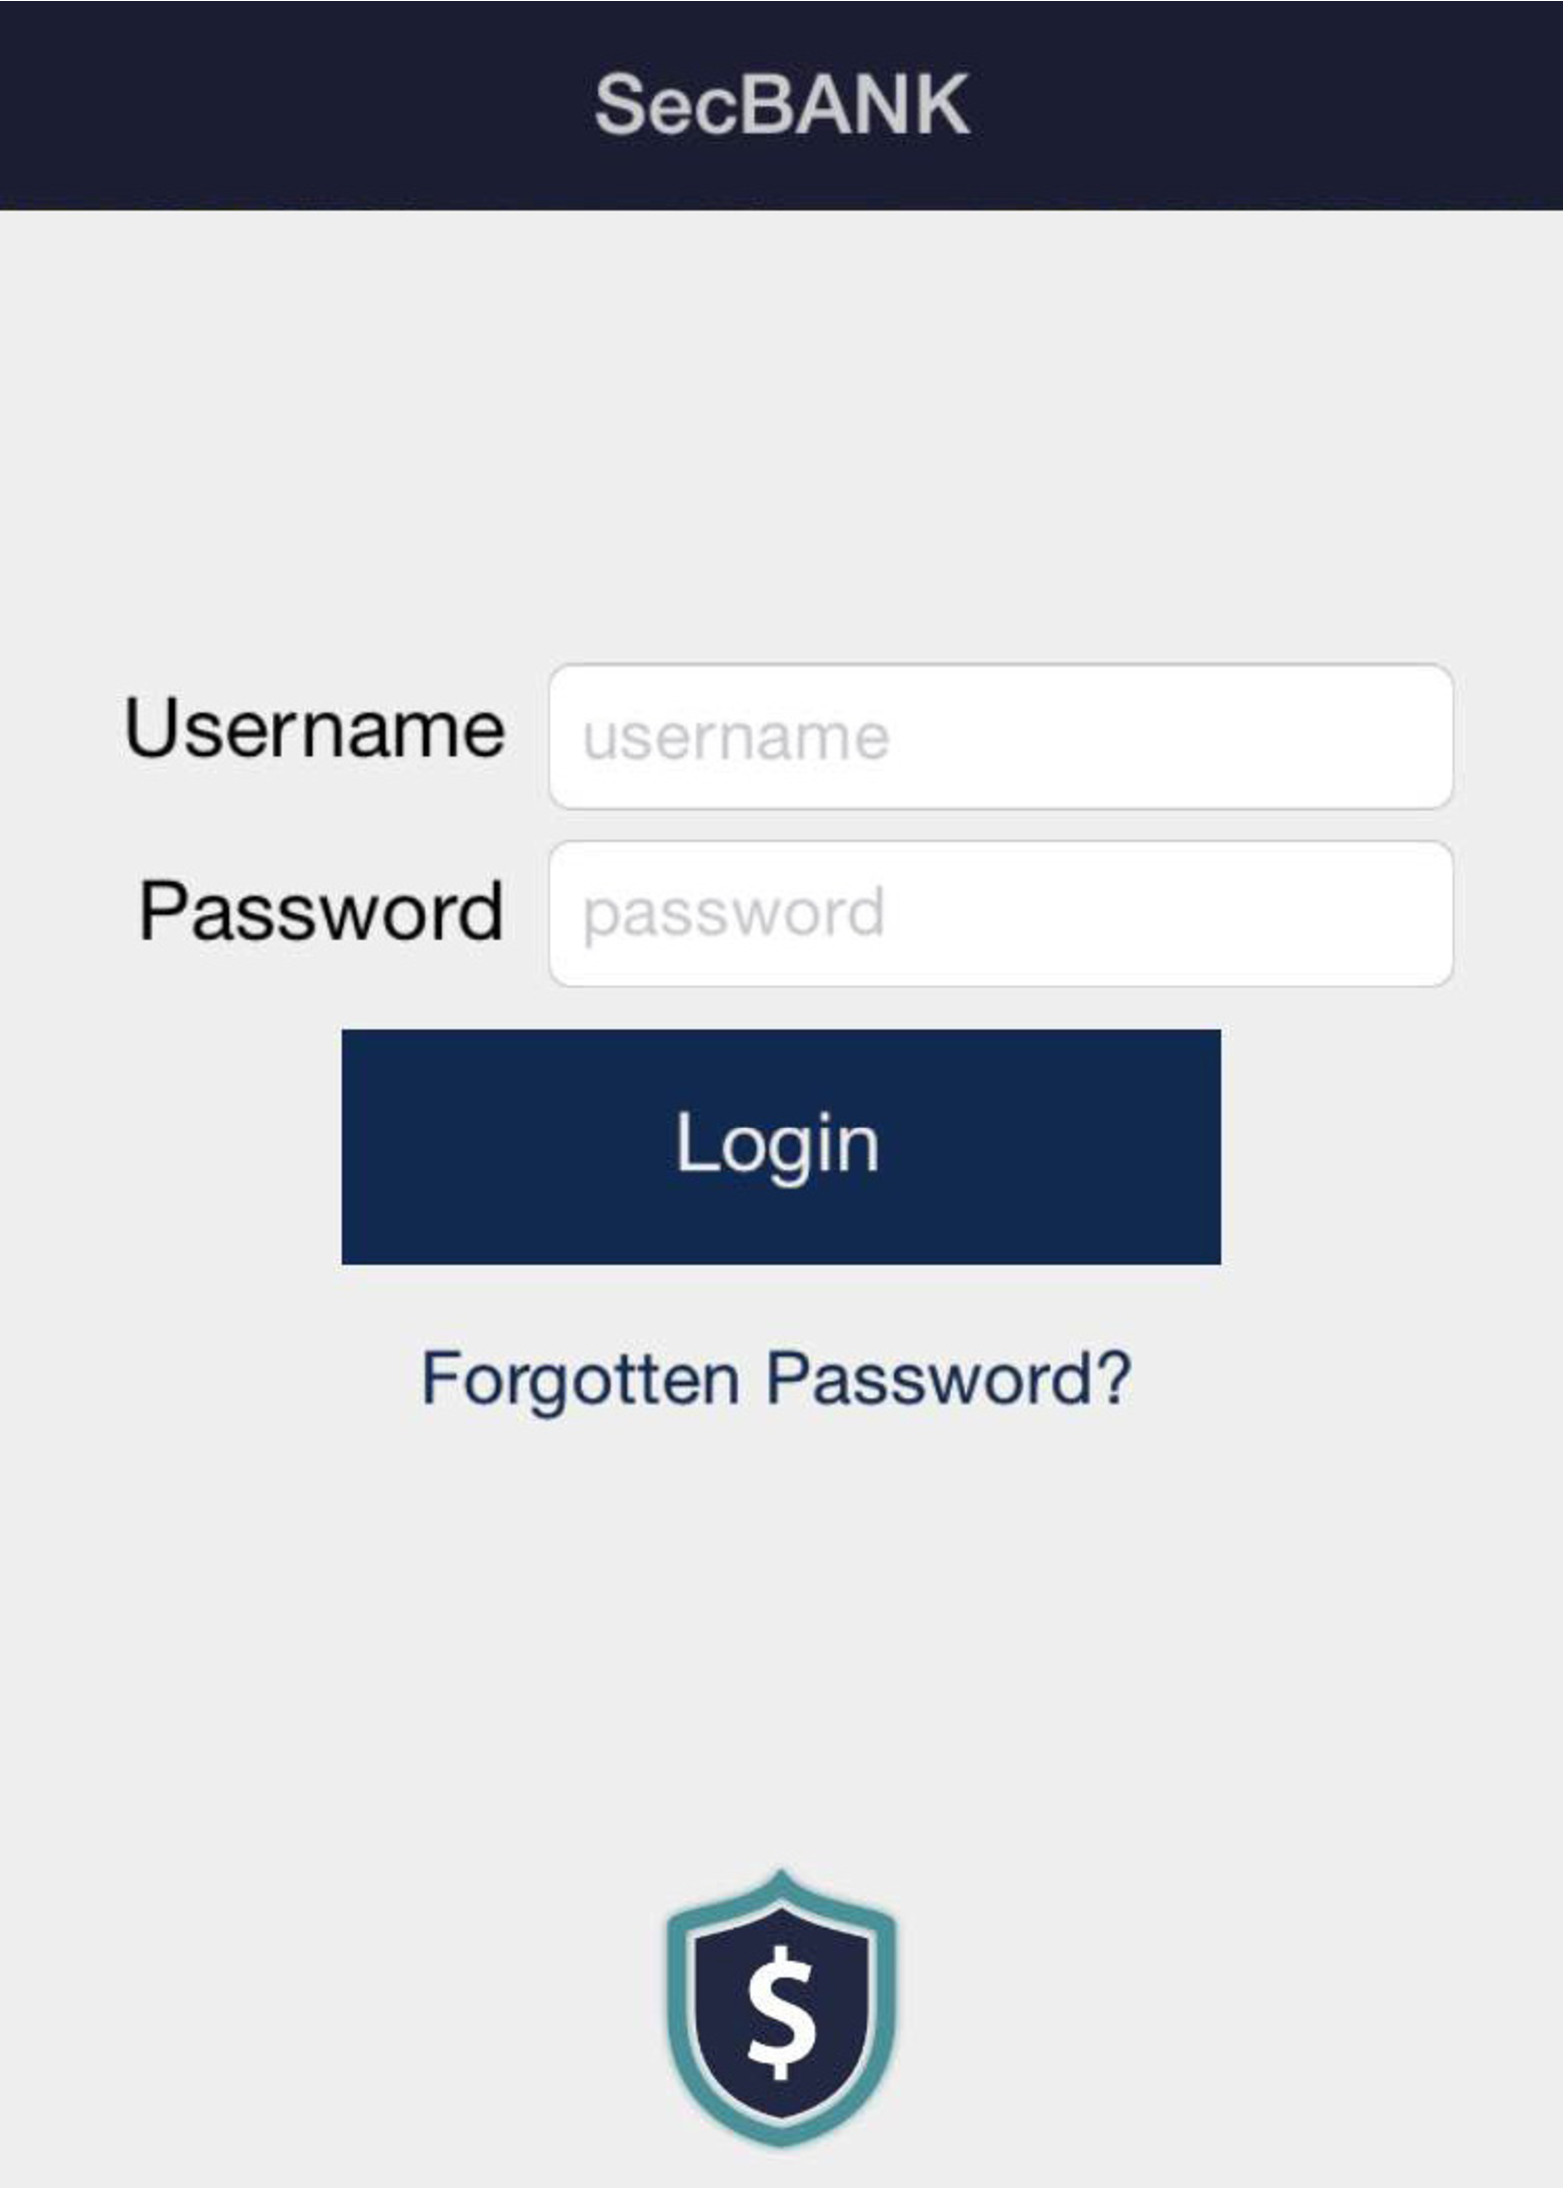
\includegraphics[width=.45\linewidth]{figures/securingphone/phishing_screen_noindicators}
    \label{app:sp_phishing_control_group}
  }
  ~
  \quad
  \subfigure[]{%
    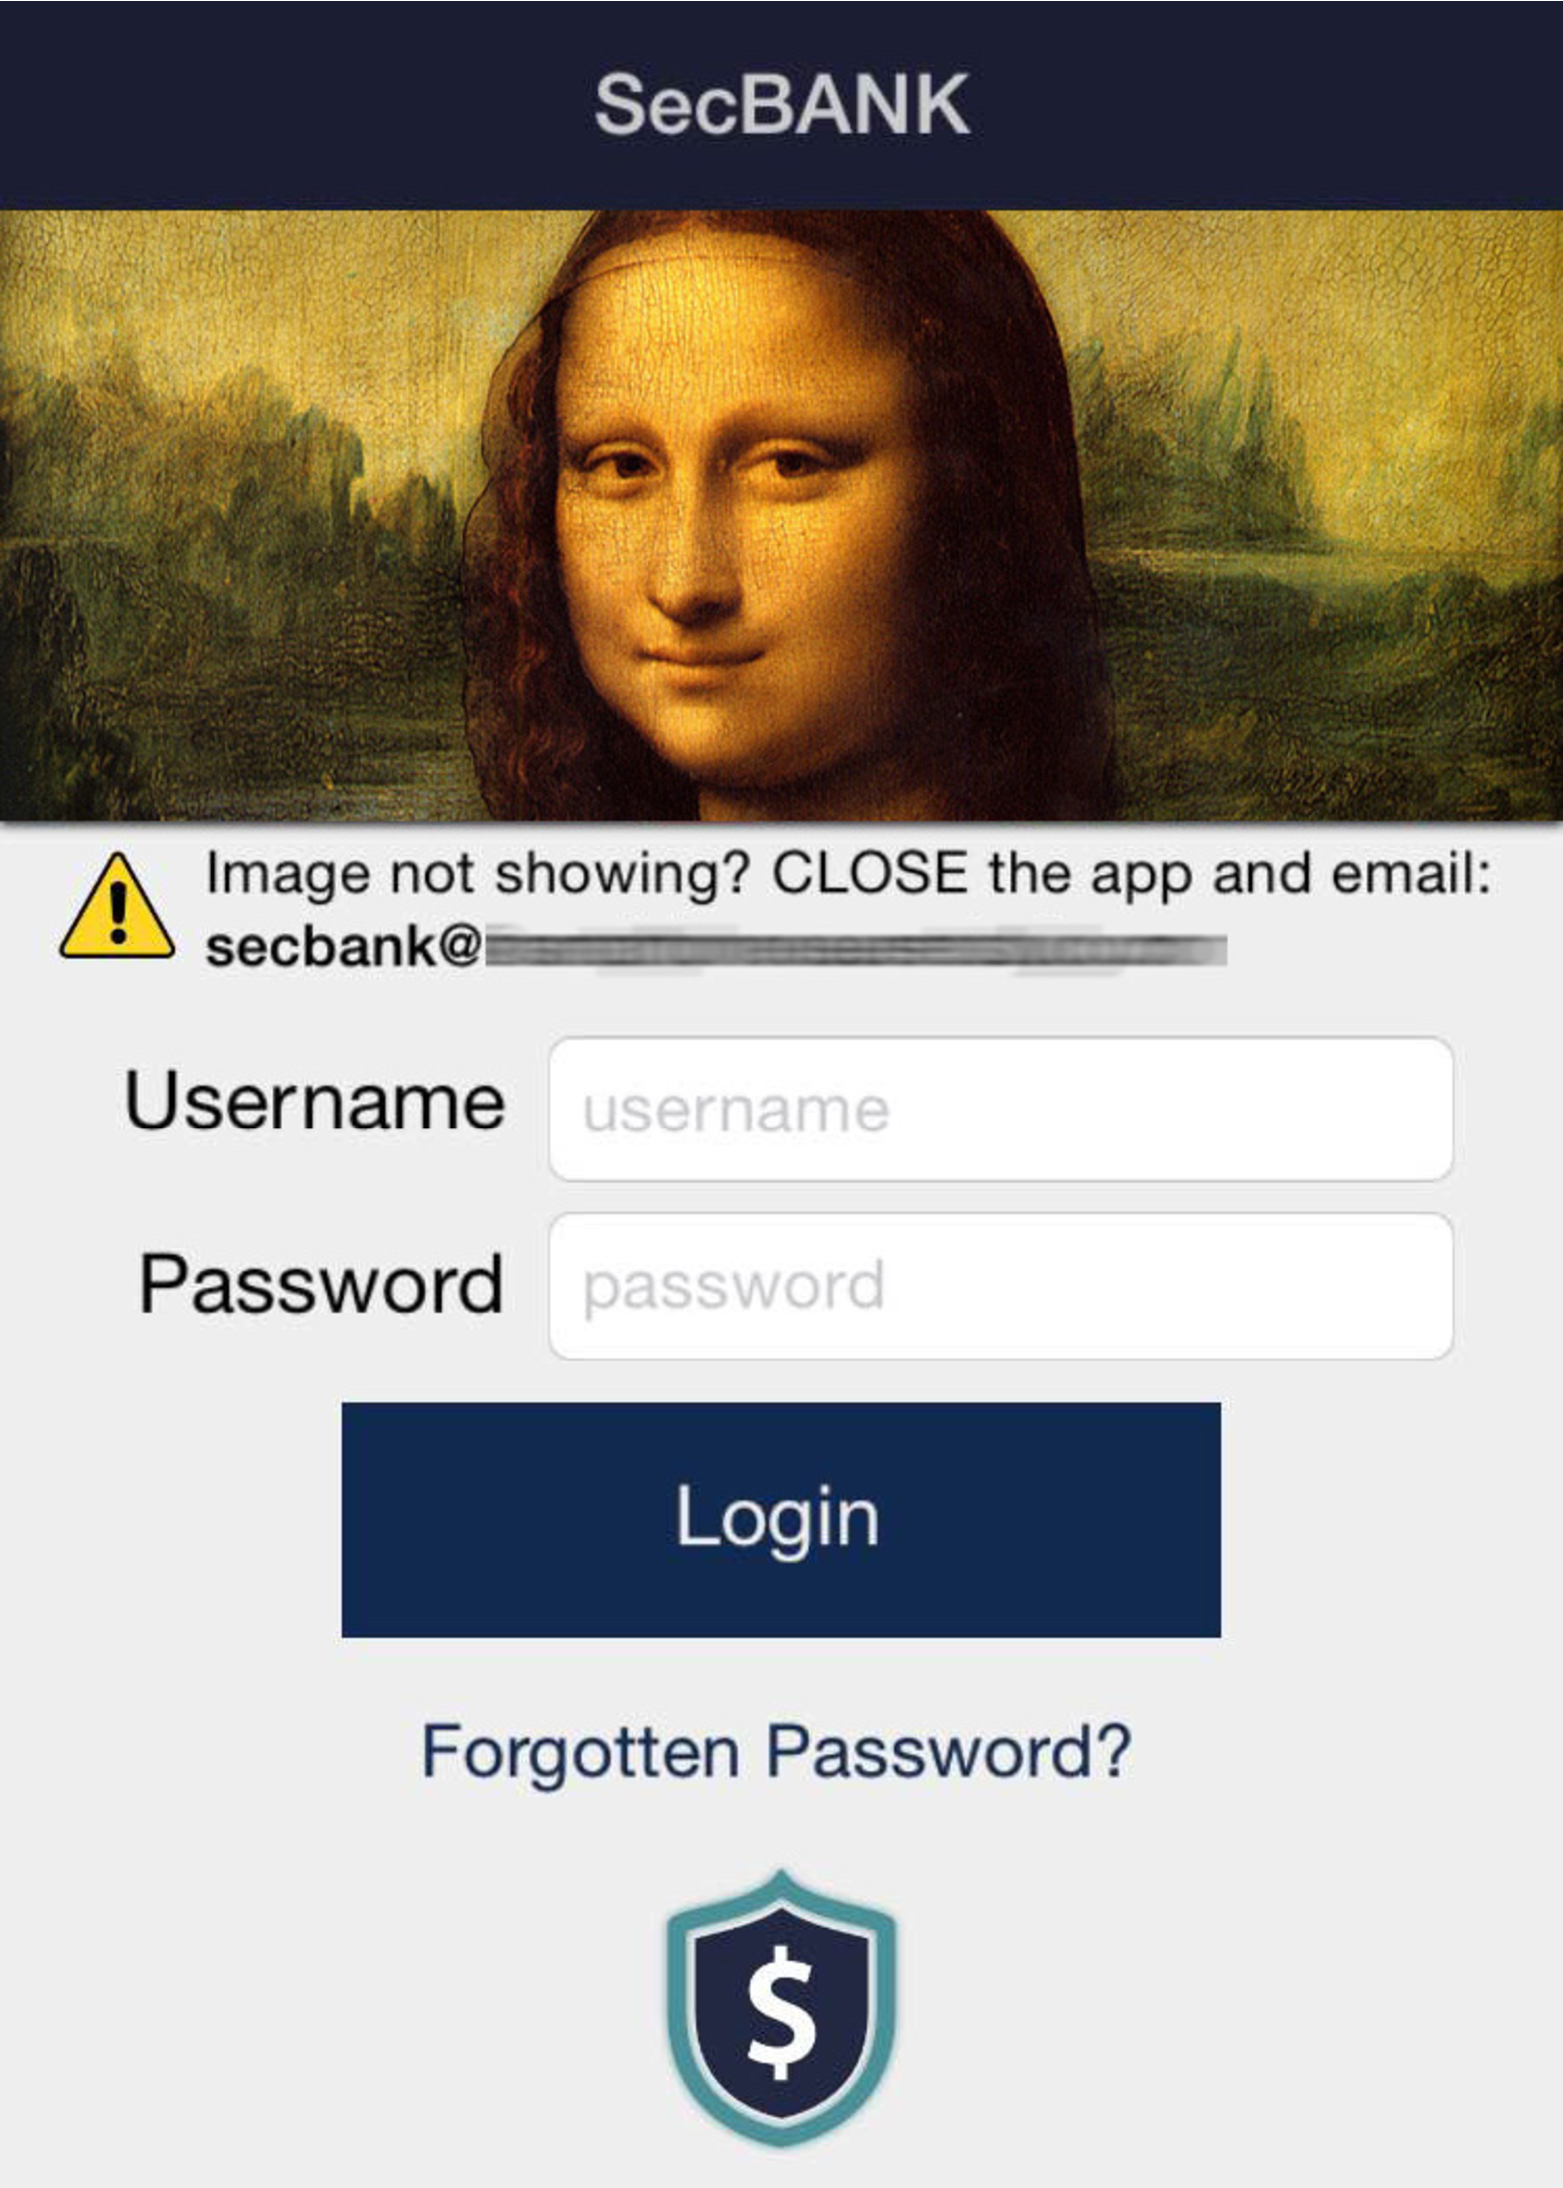
\includegraphics[width=.45\linewidth]{figures/securingphone/phishing_screen_mona}
    \label{app:sp_phishing_attack_groups}
  }
  \caption[SecBank application for the control group and the three experimental groups]{
  (a) SecBank application for the control group. The application did not use personalized indicators.
  (b) SecBank application for the three experimental groups. 
  The application displayed the personalized indicator chosen by the user on the login screen (i.e., the Mona Lisa).}
\end{figure}

The goal of our user study was to evaluate the effectiveness of personalized indicators as a phishing-detection mechanism for mobile applications.
We focused on a mobile banking scenario and implemented an application that allowed users to carry out e-banking tasks for a fictional bank called SecBank.
As no bank currently uses indicators when the user performs a login operation, an evaluation in the context of a real deployment was not possible.
The application had two components: a benign component that included the logic to log in and to carry out the banking tasks, and a malicious component that was in charge of carrying out the phishing attack. We used only one application to minimize the burden on the participants enrolling in our user study. That is, participants were asked to install only one application, rather than the banking application and another innocent-looking application that would perform the phishing attack.

In order to avoid participants focusing on the security aspects of the study, we advertised it as a user study to assess the usability of a mobile application (the full text of the advertisement e-mail can be found in Appendix~\ref{app:sp_phishing_advertising}).
We asked participants to install the SecBank application on their phones and provided them with login credentials (username and password) to access their accounts at SecBank.
We assigned each participant to either a control group that used a SecBank application without personalized indicators (Figure~\ref{app:sp_phishing_control_group}), or one of three experimental groups that used it with personalized indicators (Figure~\ref{app:sp_phishing_attack_groups}).
The experimental groups differed by the type of phishing attack. The user study lasted one week.
During the first three days, we asked participants to carry out one e-banking task per day, in order to familiarize participants with the application.
On the seventh day, we asked participants to perform a fourth e-banking task and, at this time, the malicious component of the application performed a phishing attack.
We recorded whether participants entered their credentials while under attack.

\paragraph{Ethical guidelines} We informed the participants that the
application would record their input and have access to the photo gallery on
their phones. We further explained that the application would send no personal
information to our servers. We collected the participants' email addresses to
send them instructions on how to complete the e-banking tasks. The email
addresses were deleted once the study was finished. At the end of the study, we
briefed participants about the true purpose and the methodology of the study.
We notified the ethical board of our institution which reviewed and approved
our protocol before we started the user study.

\begin{figure}[!ht]
  \centering
  \subfigure[]{%
    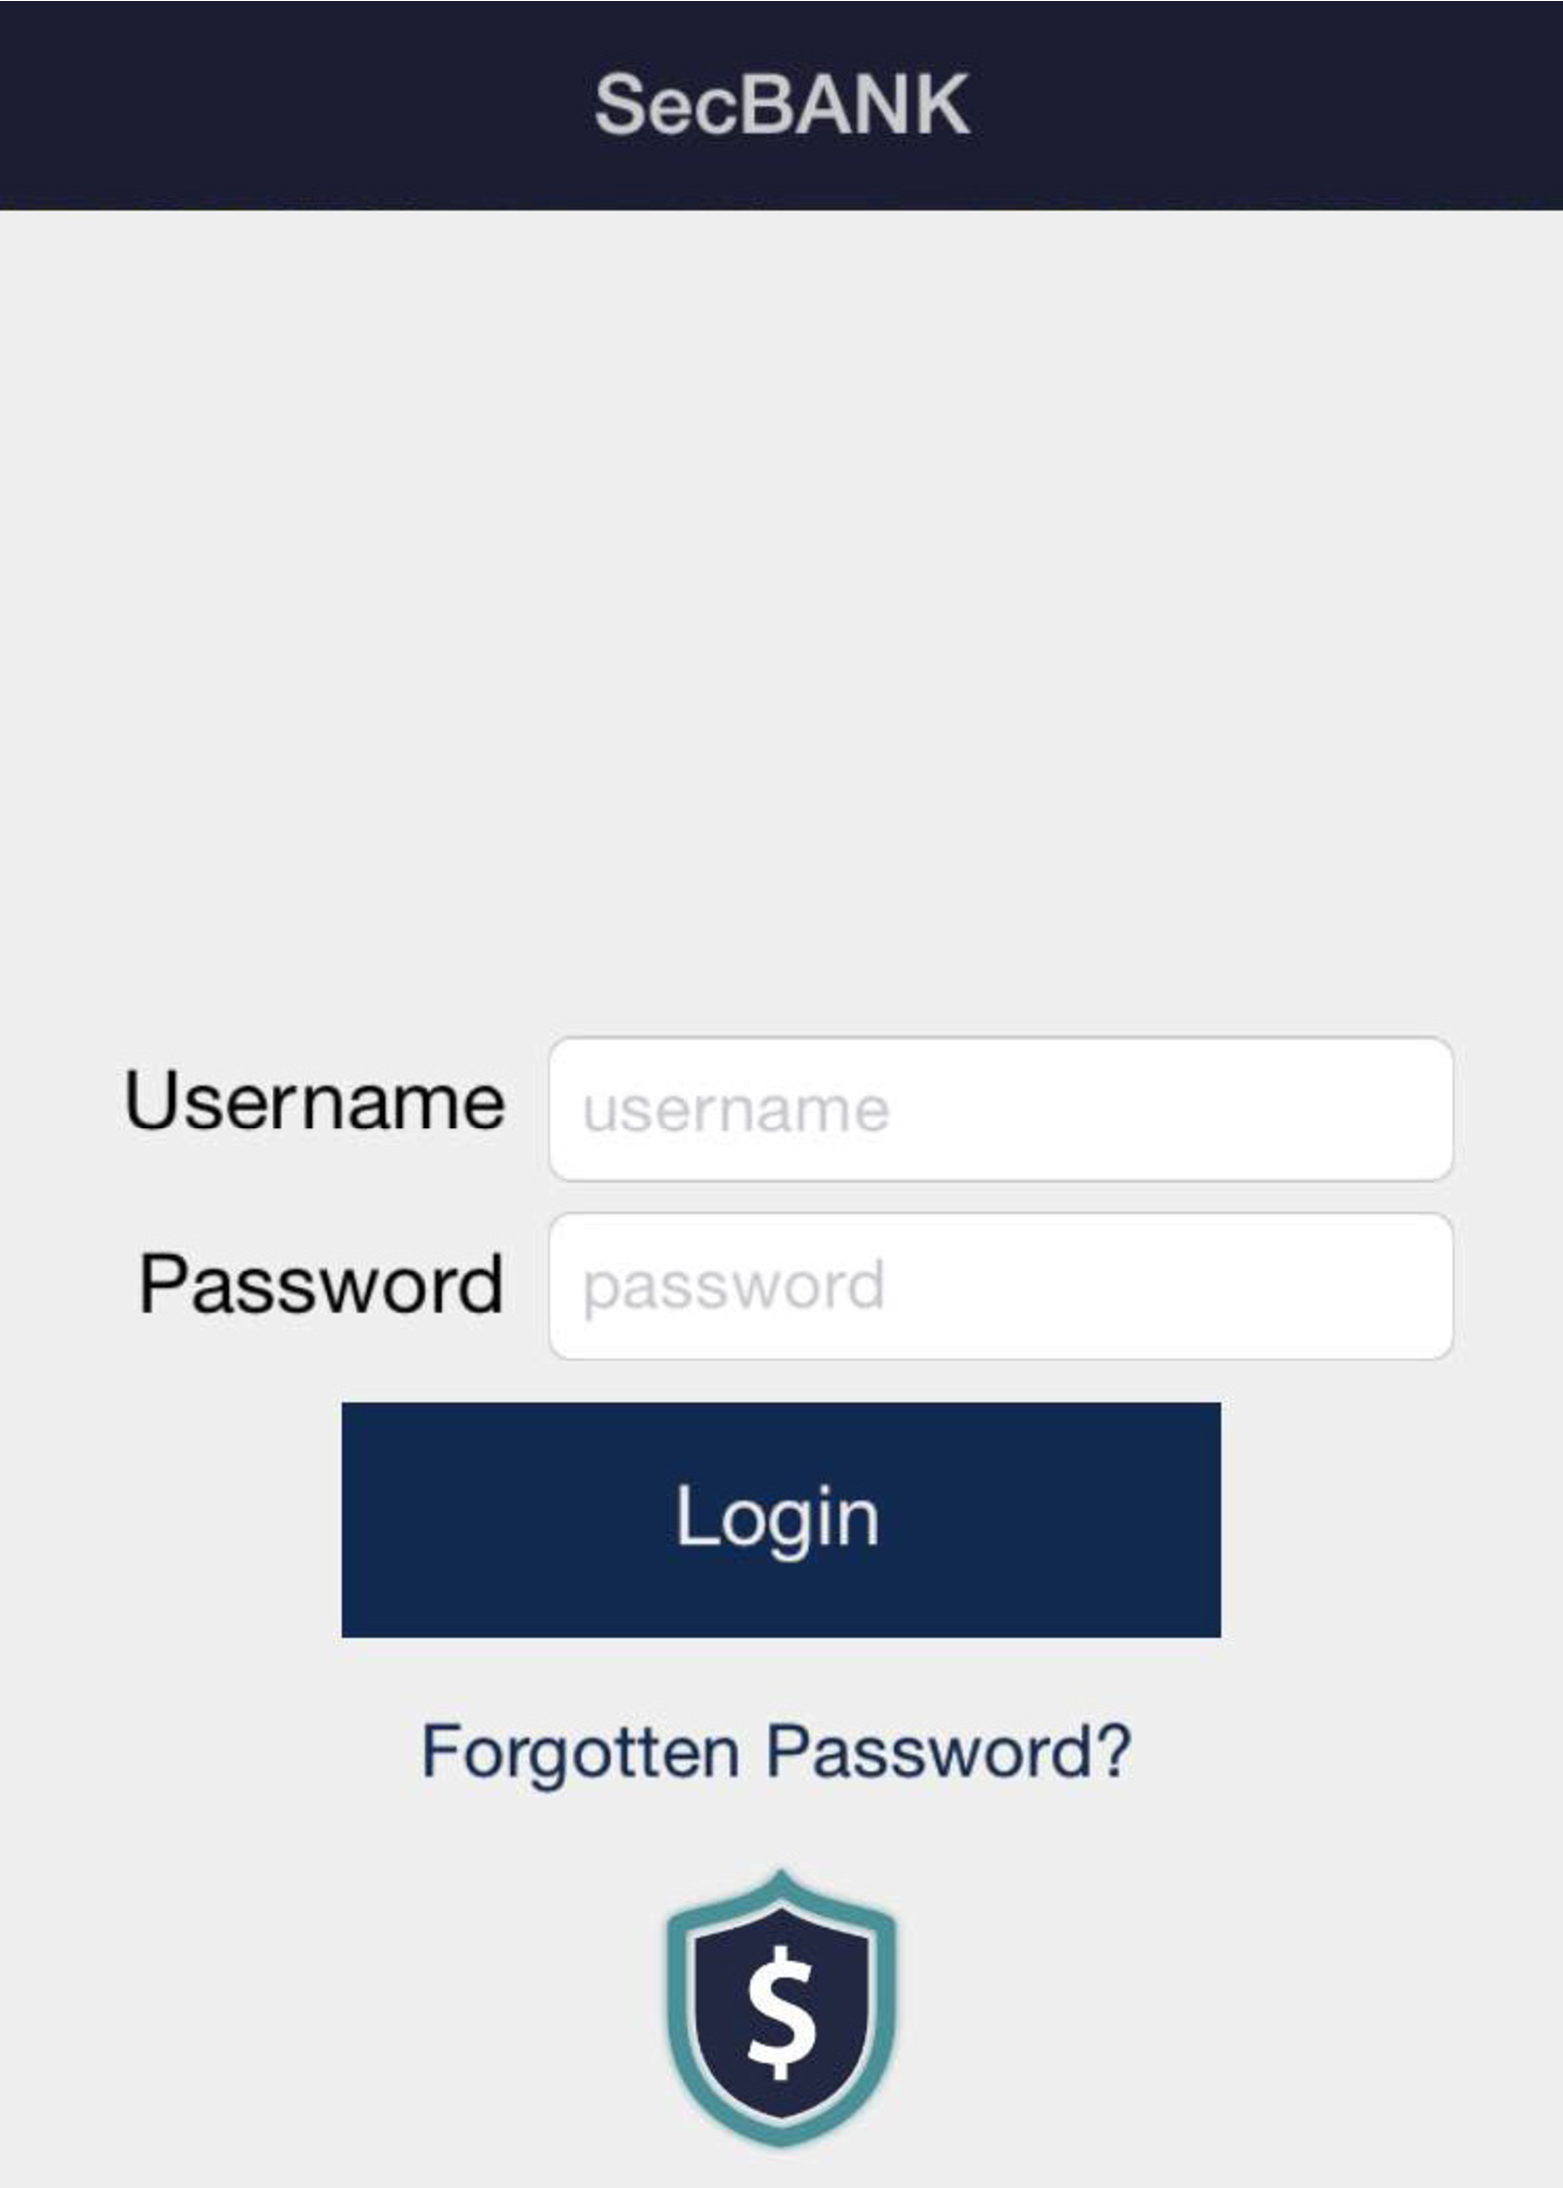
\includegraphics[width=.3\linewidth]{figures/securingphone/phishing_screen_empty}
    \label{app:sp_phishing_noimage}
  }
  ~
  \subfigure[]{%
    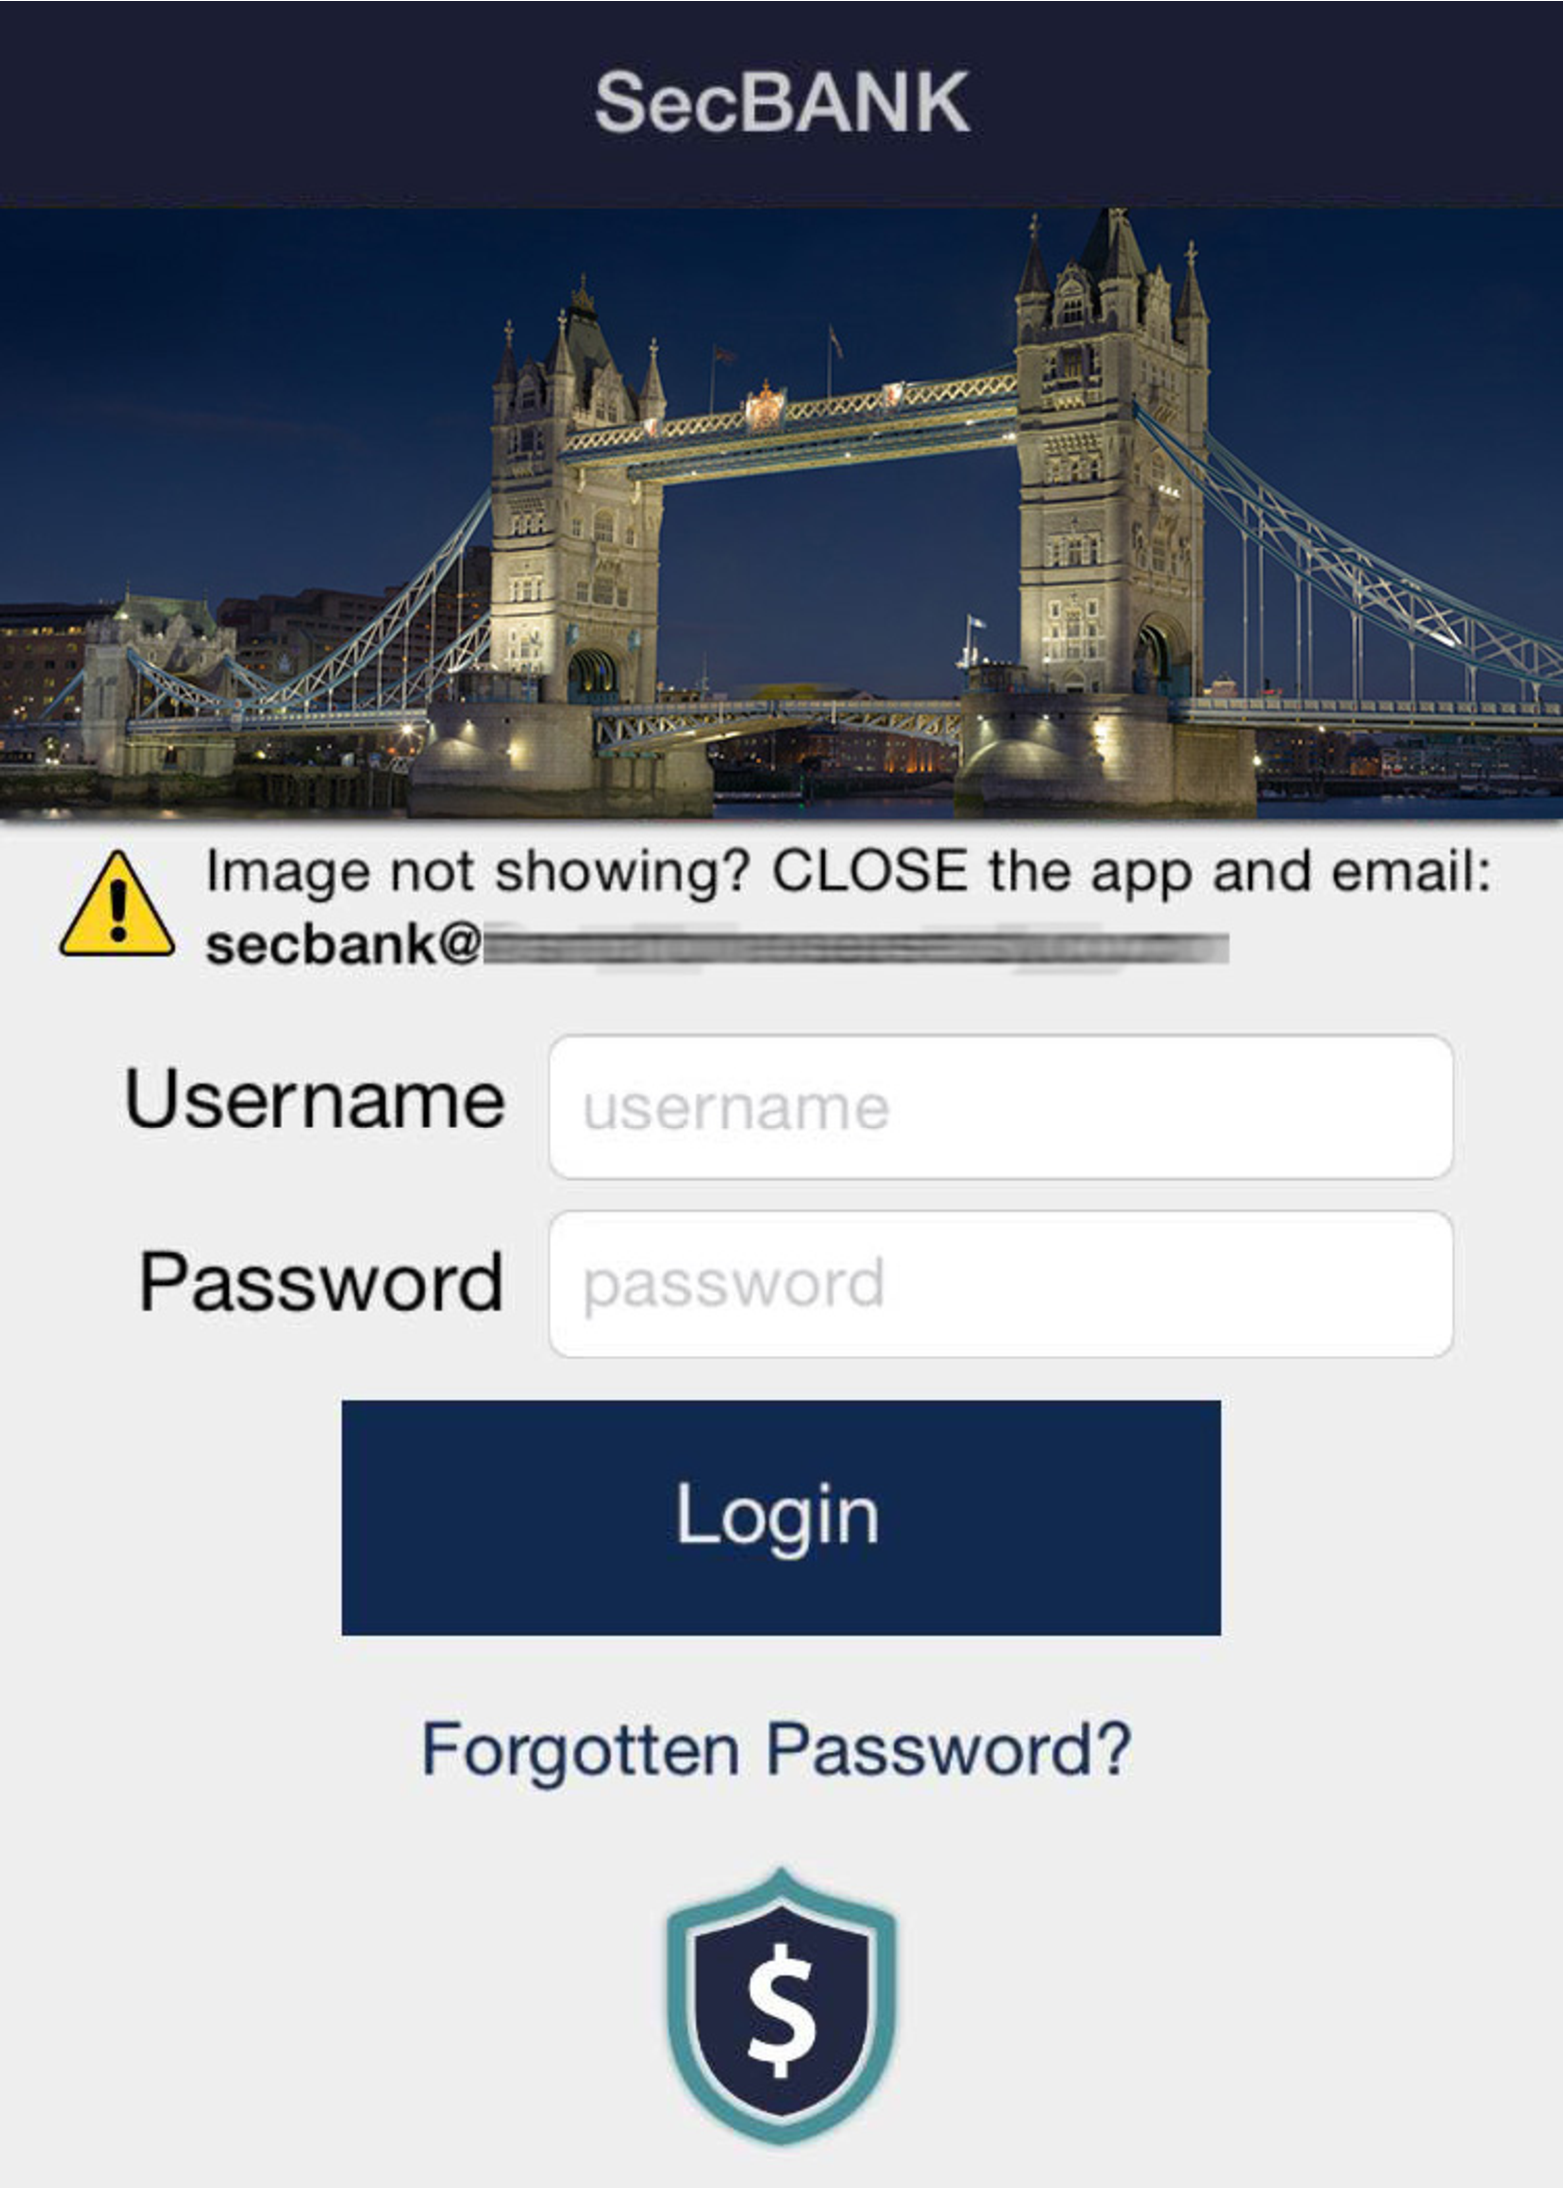
\includegraphics[width=.3\linewidth]{figures/securingphone/phishing_screen_towerbridge}
    \label{app:sp_phishing_towerbridge}
  }
  ~
  \subfigure[]{%
    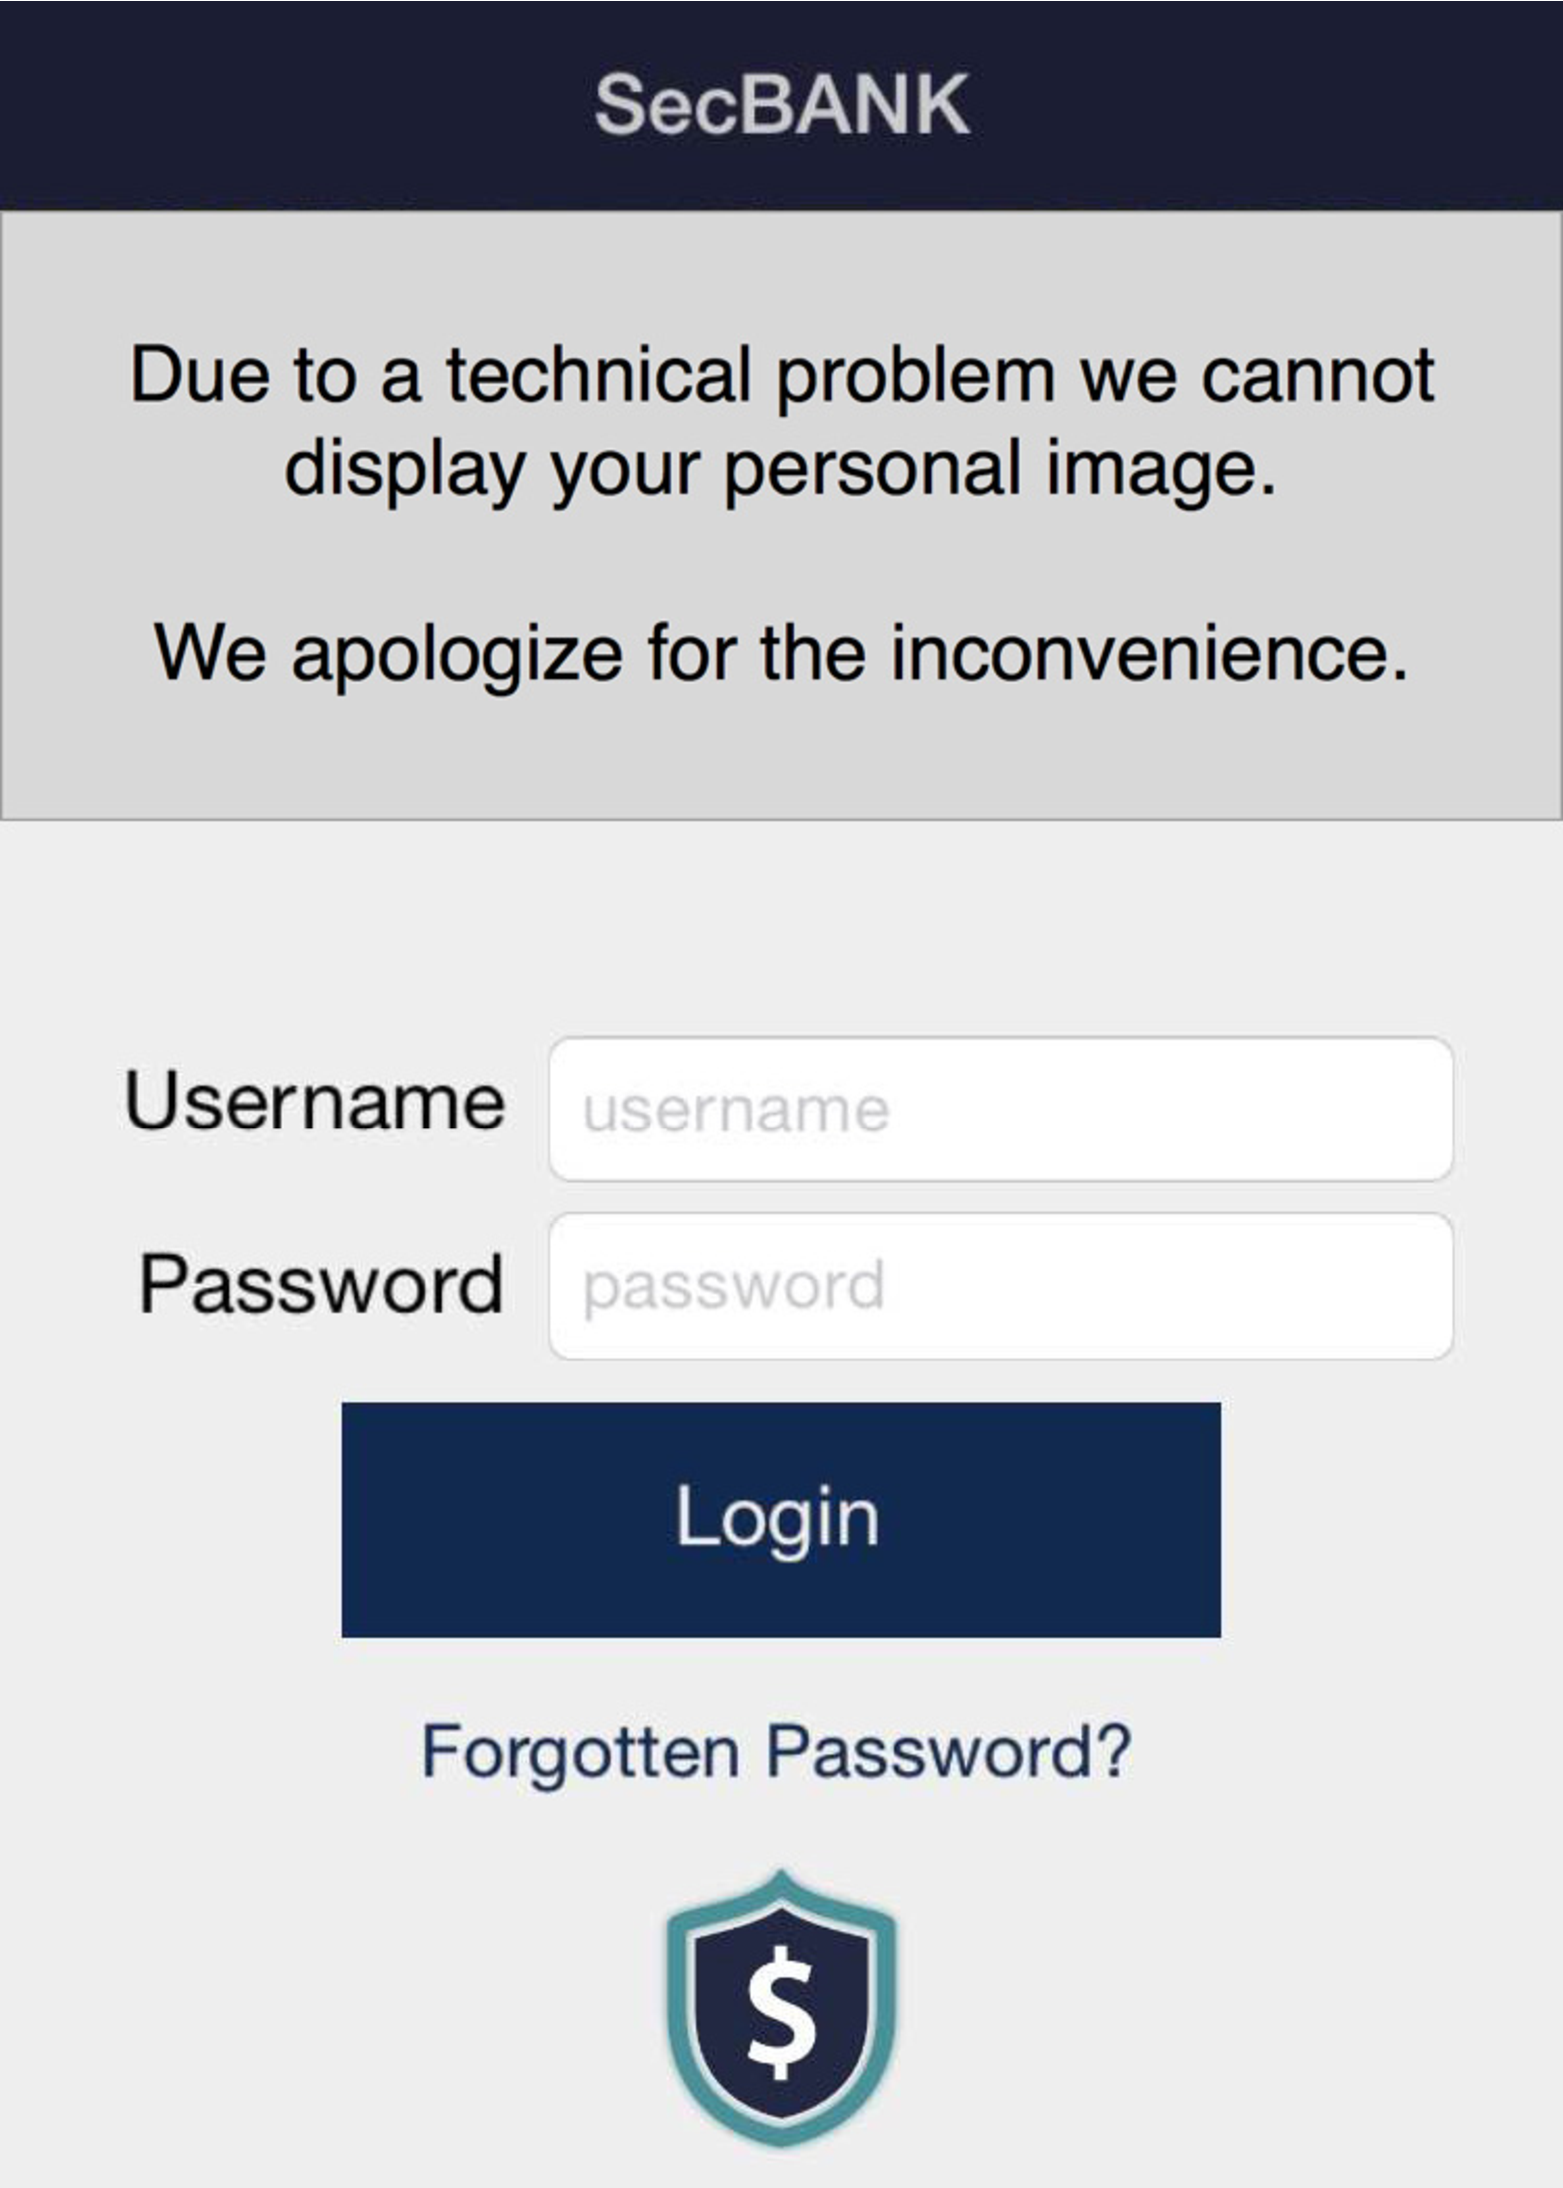
\includegraphics[width=.3\linewidth]{figures/securingphone/phishing_screen_maintenance}
    \label{app:sp_phishing_maintenance}
  }
  \caption[Different attacks presented to the three experimental groups]{
  (a) Missing-Image attack: The application does not show the indicator chosen by the user.
  (b) Random-Image attack: The application shows a random image from the local photo gallery (e.g., the Tower Bridge of London).
  (c) Maintenance attack: The application shows a message explaining that the indicator cannot be displayed due to technical reasons.
  }
\end{figure}

\subsection{Procedure}

\paragraph{Recruitment and group assignment} We recruited participants through
an email sent to all people with an account at our institute (students, faculty
and university staff). The study was advertised as a user study to ``test the
usability of a mobile banking application'' without details of the real purpose
of our design. We offered a compensation of CHF 20.- to all participants who
completed the pre-test questionnaire.

We received 465 emails from potential participants to whom we replied with a
link to an online pre-test questionnaire designed to collect email addresses
and demographic information. 301 participants filled in the pre-test
questionnaire. We assigned them to the following four groups (one control group
and three experimental groups) in a round-robin fashion:

\begin{itemize}
  \item \textbf{Control Group (A):} The application used by this group did not use personalized indicators.
  On the last day of the user study, the malicious component of the application showed a clone of the SecBank login screen, leaving the user with no visual clues to identify the phishing attack.
  \item \textbf{Missing-Image Group (B):} The application used by this group supported personalized indicators.
  On the last day of the user study, the malicious component of the application performed a phishing attack and showed the SecBank login screen without the indicator (Figure~\ref{app:sp_phishing_noimage}).
  \item \textbf{Random-Image Group (C):} The application used by this group supported personalized indicators.
  On the last day of the user study, the malicious component of the application performed a phishing attack and showed the SecBank login screen with a photo randomly chosen from the local photo gallery. The photo displayed was different from the one chosen by the user as the personalized indicator (Figure~\ref{app:sp_phishing_towerbridge}).
  \item \textbf{Maintenance Group (D):} The application used by this group supported personalized indicators.
  On the last day of the user study, the malicious component of the application performed a phishing attack and showed the SecBank login screen with an ``under maintenance'' notification in place of the indicator chosen by the user (Figure~\ref{app:sp_phishing_maintenance}).
\end{itemize}

We sent an email to all participants who completed the pre-test questionnaire
with a link to a webpage from which they could install the SecBank
application (the full text of this e-mail can be found in Appendix~\ref{app:sp_phishing_selectedemail}).
Participants in the Control Group (A) were directed to a webpage
where we only explained how to install the application.
Participants in experimental groups B, C, and D were directed to a webpage that
also explained the concept of personalized indicators. The
webpage advised that participants should not enter their login credentials if
the application was not showing the correct indicator (the text of the webpage can be found in Appendix~\ref{app:sp_phishing_priming}).
The instructions were similar to the ones used in banking websites that deploy indicators~\cite{boa,vanguard}.
276 participants visited the webpages and installed the SecBank application on their devices.
After installation, the SecBank application for groups B, C, and D showed explanatory overlays to guide participants in choosing a personalized indicator from their photo gallery.

\paragraph{Tasks} The study lasted one week. Participants were asked to
perform four e-banking tasks on days 1, 2, 3, and 7. We sent instructions via email and asked participants to complete the task within
24 hours (The e-mail text of the first task can be found in Appendix~\ref{app:sp_phishing_taskemail}. The following tasks had similar e-mail structure and text.).
The tasks were the following:

\begin{itemize}
	\item \textbf{Task 1} (Day 1): ``Transfer \$200 to Anna Smith.''
	\item \textbf{Task 2} (Day 2): Download the bank statement from the ``Account Overview'' tab.
	\item \textbf{Task 3} (Day 3): Activate the credit card from the ``Cards'' tab.
	\item \textbf{Task 4} (Day 7): Transfer \$100 to ``George White''.
\end{itemize}

The goal of tasks 1--3 was to help participants to become familiar with the SecBank application.
We sent the instructions to perform the last task four days after (including a weekend) the completion of task 3.
During this last task, the malicious component of the application performed a phishing attack on all participants.
Participants in the Control Group (A) saw a login screen that matched that of their SecBank application.
Participants in the Missing-Image Group (B) saw a login screen similar to the one of SecBank, but without any personalized indicator (Figure~\ref{app:sp_phishing_noimage}).
Participants in the Random-Image Group (C) saw a login screen similar to SecBank, but with a random image from their photo gallery (e.g., the Tower Bridge as shown in Figure~\ref{app:sp_phishing_towerbridge}).
Finally, participants in the Maintenance Group (D) saw a message explaining that for technical problems the indicator could not be displayed (Figure~\ref{app:sp_phishing_maintenance}).

\begin{table}[!ht]
    \begin{center}
        \scalebox{.9}{
        \begin{tabu}{|l|c|} \hline
          \multicolumn{2}{|l|}{Gender} \\ \hline
          Male & 150 (68\%) \\
          Female & 71 (32\%) \\ \hline
          \multicolumn{2}{|l|}{Age} \\ \hline
          Up to 20 & 43 (20\%) \\
          21 -- 30 & 164 (74\%) \\
          31 -- 40 & 9 (4\%) \\
          41 -- 50 & 3 (1\%) \\
          51 -- 60 & 0 (0\%) \\
          Over 60 & 2  (1\%) \\ \hline
          \multicolumn{2}{|l|}{Use smartphone to read emails} \\ \hline
          Yes & 214 (97\%) \\
          No & 7 (3\%) \\ \hline
          \multicolumn{2}{|l|}{Use smartphone for social networks} \\ \hline
          Yes & 218 (99\%) \\
          No & 3 (1\%) \\ \hline
          \multicolumn{2}{|l|}{Use smartphone for e-banking} \\ \hline
          Yes & 97 (44\%) \\
          No & 124 (56\%) \\ \hline
%          \multicolumn{2}{|l|}{Smartphone display size (diagonal)} \\ \hline
%          $< 4$in & 64 (29\%) \\
%          $< 4.5$in & 131 (59\%) \\
%          $< 5$in & 26 (12\%) \\ \hline
        \end{tabu}}
    \end{center}
    \caption[Demographic information of the 221 participants that completed all tasks]{Demographic information of the 221 participants that completed all tasks.}
    \label{tab:sp_phishing_demographics}
\end{table}


\subsection{Results}

Out of 276 participants that installed the application, 221 completed all
tasks. We provide their demographics and other information collected during the
pre-test questionnaire in Table~\ref{tab:sp_phishing_demographics}. The majority of the
participants were male (68\%) and thirty years old or younger (94\%). Most participants
used their smartphone to read emails (97\%) and to access social networks (99\%).
Slightly less than half of the participants (44\%) used their smartphones for
mobile banking.

\begin{table}[!ht]
    \begin{center}
      \scalebox{.9}{
      {\tabulinesep=.4mm
        \setlength{\tabcolsep}{1.5mm}
        \begin{tabu}{|m{2.9cm}|C{2.2cm}|C{2.2cm}|} \hline
          & Attack not successful & Attack successful \\ \hline
          Control Group (A) & 0 (0\%) & 56 (100\%) \\ \hline \hline
          Missing-Image Group (B) & 30 (55\%) & 25 (45\%) \\ \hline
          Random-Image Group (C) & 23 (41\%) & 33 (59\%) \\ \hline
          Maintenance Group (D) & 29 (54\%) & 25 (46\%) \\ \hline \hline
          Experimental groups combined & 82 (50\%) & 83 (50\%) \\ \hline
        \end{tabu}}}
    \end{center}
    \caption[Success rate of the phishing attack]{Success rate of the phishing attack.}
    \label{tab:sp_phishing_primary}
\end{table}

\begin{table}[t]
    \begin{center}
      \scalebox{.9}{
      {\tabulinesep=.4mm
        \setlength{\tabcolsep}{1.5mm}
        \begin{tabu}{|m{2.5cm}|C{2.2cm}|C{2.2cm}|} \hline
          & Attack not successful & Attack successful \\ \hline
          \multicolumn{3}{|l|}{Gender} \\ \hline
          Male & 59 (52\%) & 54 (48\%) \\ \hline
          Female & 23 (44\%) & 28 (56\%) \\ \hline
          \multicolumn{3}{|l|}{Age} \\ \hline
          Up to 20 & 15 (43\%) & 20 (57\%) \\ \hline
          21 -- 30 & 57 (48\%) & 61 (52\%) \\ \hline
          31 -- 40 & 6 (86\%) & 1 (14\%) \\ \hline
          41 -- 50 & 2 (67\%) & 1 (33\%) \\ \hline
          51 -- 60 & 0 (0\%) & 0 (0\%) \\ \hline
          Over 60 & 2 (100\%) & 0 (0\%) \\ \hline
          \multicolumn{3}{|l|}{Use smartphone for e-banking} \\ \hline
          Yes & 41 (54\%) & 35 (46\%) \\ \hline
          No & 41 (46\%) & 48 (54\%) \\ \hline
          \multicolumn{3}{|l|}{Smartphone display size (diagonal)} \\ \hline
          up to $4$in & 28 (58\%) & 20 (42\%) \\ \hline
          from  $4$in to $4.5$in & 44 (45\%) & 54 (55\%) \\ \hline
          from $4.6$in to $5$in & 10 (53\%) & 9 (47\%) \\ \hline
        \end{tabu}}}
    \end{center}
    \caption[Success rate of the phishing attack in relation to gender, age, familiarity with mobile banking, and smartphone display size]{Success rate of the phishing attack in relation to gender, age, familiarity with mobile banking, and smartphone display size.}
    \label{tab:sp_phishing_secondary}
\end{table}

The 221 participants that completed all tasks were distributed as follows: 56
in the Control Group (A), 55 in the Missing-Image Group (B), 56 in the
Random-Image Group (C), and 54 in the Maintenance Group
(D).\footnote{We note that, by chance, the participants that dropped out of the study were almost evenly distributed among the four groups.}

\paragraph{Indicator effectiveness} Table~\ref{tab:sp_phishing_primary} shows the success rates for the phishing attack during Task 4.
All of the 56 participants in the Control Group (A) fell for the attack (i.e., all participants entered their login credentials to the phishing application).
83 out of 165 (50\%) attacks in the experimental groups B, C, and D were successful.

To analyze the statistical significance of these results we used the following
null hypothesis: ``there will be no difference in the attack success rate between users that use personalized indicators and users that do not use personalized indicators''. A Chi-square test showed that the difference was statistically
significant ($\chi^2(3,N = 221) = 46.96, p < 0.0001$) and thus the null hypothesis
can be rejected. We conclude that, in our user study, the deployment of security indicators decreased the attack success rate and improved phishing detection.

\paragraph{Difference between attacks}
A closer look at the performance of participants in groups B, C, and D reveals that:
30 out of 55 participants in the Missing-Image Group (B),
23 out of 56 participants in the Random-Image Group (C), and
29 out of 54 participants in the Maintenance Group (D) retained from logging in.

To analyze the success rates of the different attack types we used the
following null hypothesis:
``the three attack types we tested are equally successful''.
A Chi-squared test showed no statistically
significant difference in the attack success rates, and
thus we fail to reject the null hypothesis ($\chi^2(2,N = 165) = 2.53, p = 0.282$).
We conclude that in our test setup the three attacks were equally successful and, therefore, indicators worked as well in all three scenarios.

\paragraph{Other factors} We performed post hoc analysis of our dataset to
understand if there were any relationship between the attack success rate and
gender ($\chi^2(1,N = 221) = 0.99, p = 0.319$), age group ($\chi^2(4,N = 221) =
8.36, p = 0.079$), smartphone display size ($\chi^2(2,N = 221) = 5.40, p =
0.369$) or familiarity with mobile banking ($\chi^2(1,N = 221) = 1.98, p =
0.160$). We did not find any statistical significance for any of the factors we
considered. Table~\ref{tab:sp_phishing_secondary} provides the results break-down.

Finally, we report the mean time spent by participants setting up the
personalized indicator or logging in. The mean time spent setting up the
indicator for participants that did not fall victim to the attack was 43s
($\pm$28s); the mean time for participants that fell for the attack was 46s
($\pm$28s). The mean time spent on the login screen for participants that did
not fall victim to the attack was 18s ($\pm$14s); the mean time for
participants that fell for the attack was 14s ($\pm$10s). The distribution of
the times spent while setting up the indicator and while logging in are shown
in Figure~\ref{fig:sp_phishing_distindicator} and Figure~\ref{fig:sp_phishing_distlogin}, respectively.

% Although we do not have statistical analysis of this difference, there appears to \todo{fill me}

% Our results show that participants that did not fell victim of the attack did
% not spend a significantly longer time on the login screen compared to
% participants that fell for the attack.
% We conclude, therefore, that phishing attacks may be quickly detected by using personalized indicators.

\begin{figure}[!ht]
  \centering
  \subfigure[Personal indicator setup] {%
    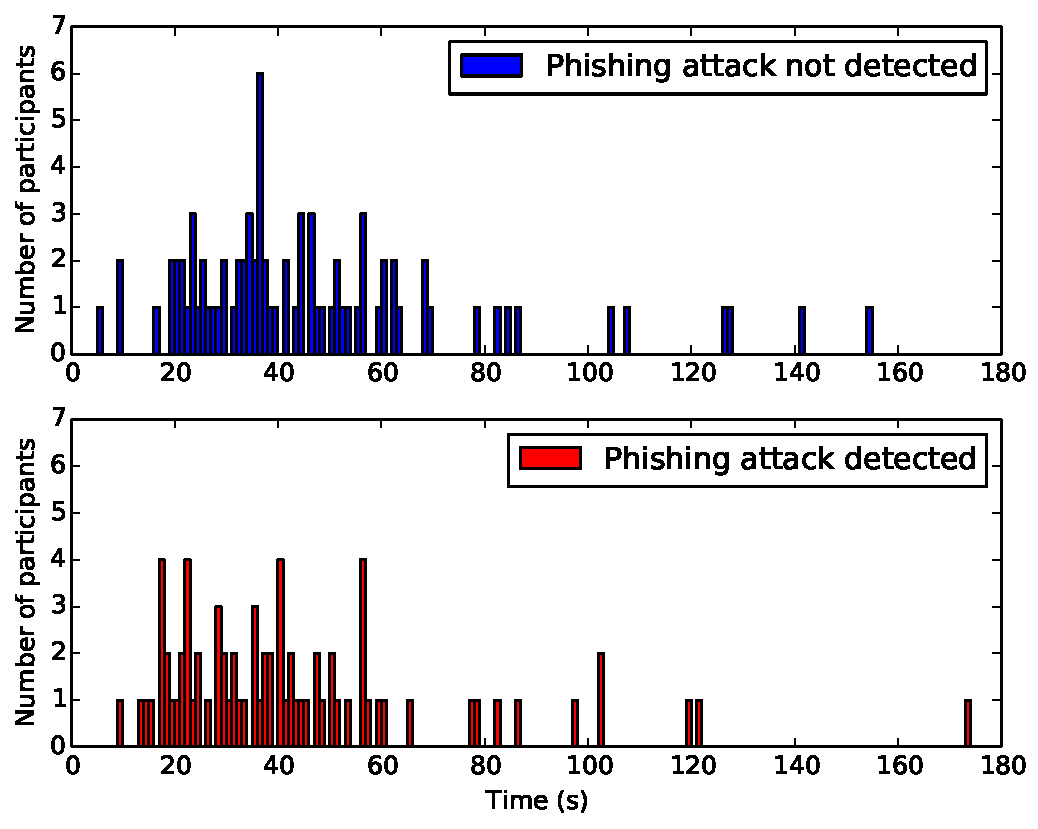
\includegraphics[width=.7\linewidth]{figures/securingphone/phishing_indicator}
    \label{fig:sp_phishing_distindicator}
  } \\
  \subfigure[Login screen]{%
    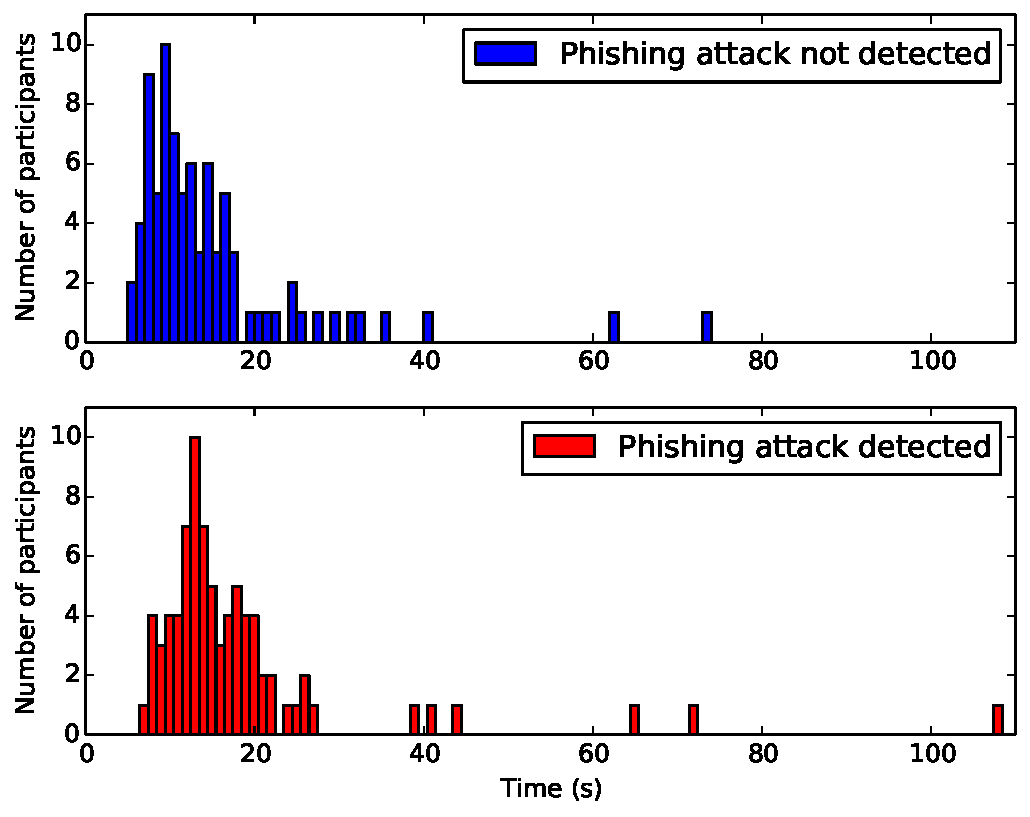
\includegraphics[width=.7\linewidth]{figures/securingphone/phishing_login}
    \label{fig:sp_phishing_distlogin}
  }
  \caption[Distribution of the time spent by participants setting up the personalized indicator and logging into the SecBank application]{Distribution of the time spent by participants setting up the personalized indicator (a) and logging into the SecBank application (b).}
\end{figure}

\subsection{Post-test questionnaire}

\begin{figure}[!ht]
	\centering
	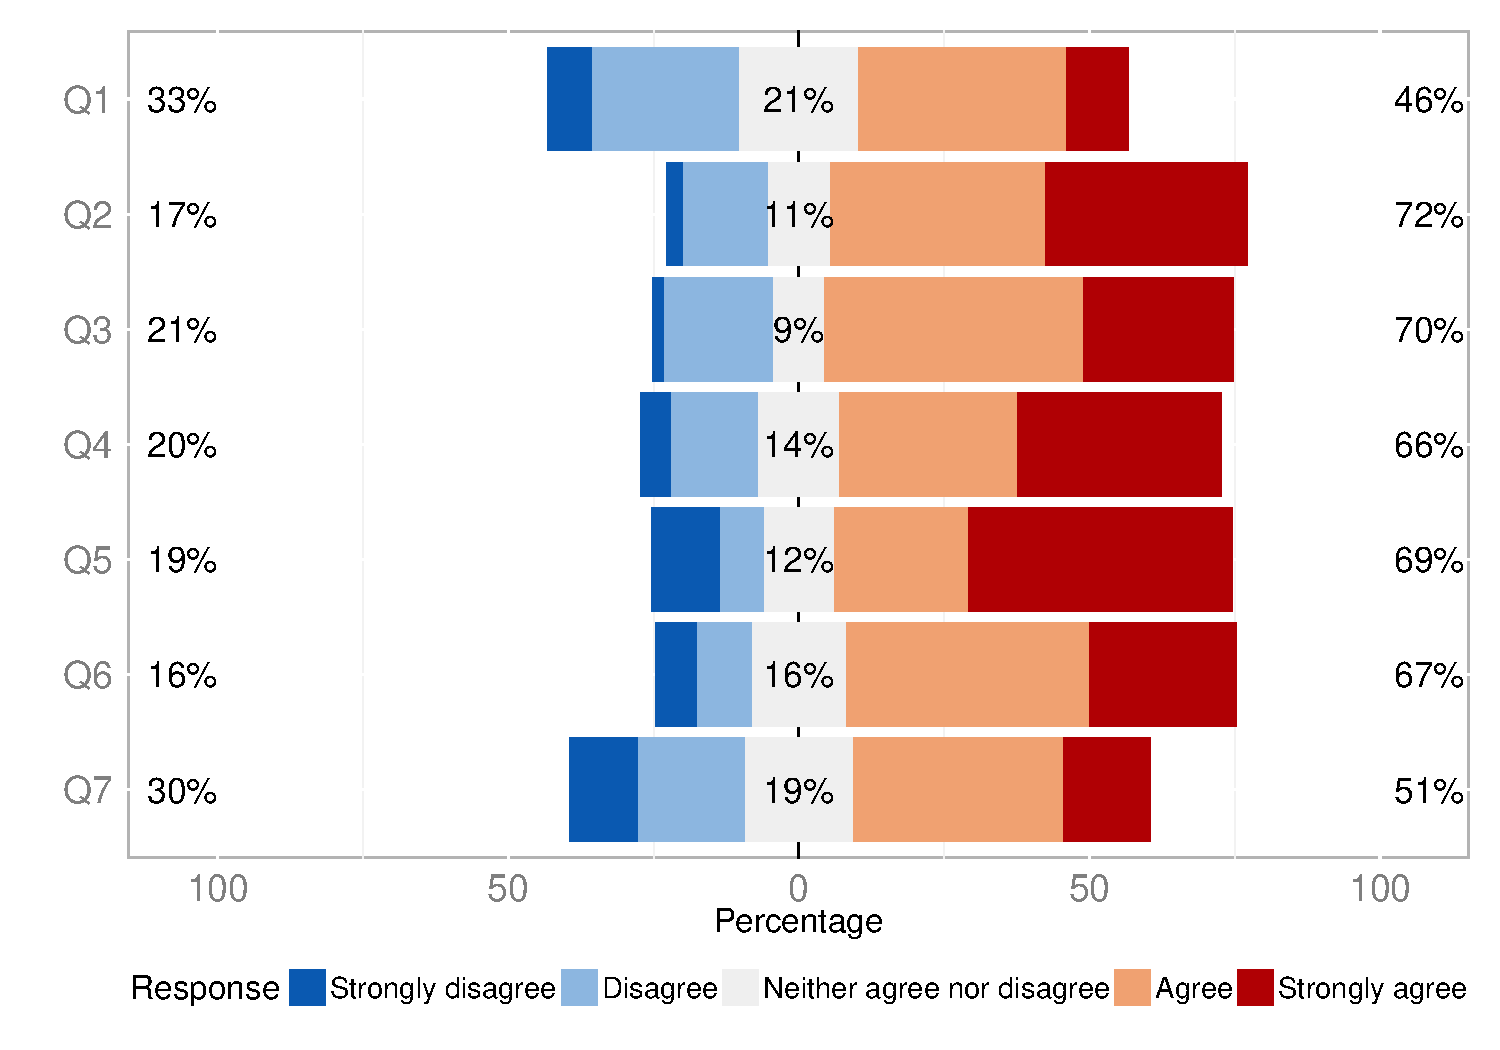
\includegraphics[width=.9\linewidth]{figures/securingphone/phishing_composite_likert}
	\caption[Answers to the post-test questionnaire]{
    Answers to the post-test questionnaire.
    Items Q1--Q4 were answered by all participants.
    Items Q5--Q7 were answered only by participants in the experimental groups (B, C, and D).
	Percentages on the left side include participants that answered ``Strongly disagree'' or ``Disagree''.
	Percentages in the middle account for participants that answered ``Nor agree, nor disagree''.
	Percentages on the right side include participants that answered ``Agree'' or ``Strongly agree''.}
	\label{plot:sp_phishing_compositelikert}
\end{figure}


Participants that completed all tasks received a post-test questionnaire with the following items:

\begin{itemize}
\setlength\itemsep{-1.2mm}
\item[Q1]\emph{I am concerned about malware on my smartphone}
\item[Q2]\emph{I am concerned about the secrecy of my password for mobile banking}
\item[Q3]\emph{I am concerned about the secrecy of my password for my email account}
\item[Q4]\emph{I am more concerned about the secrecy of my mobile banking password compared to my email password}
\item[Q5]\emph{During the study, I have made sure that my personal image was showing before entering my username and password}
\item[Q6]\emph{The login mechanism using personal images was intuitive and user-friendly}
\item[Q7]\emph{I would use personal images in other applications}
\end{itemize}


All participants answered items Q1--Q4.
Figure~\ref{plot:sp_phishing_compositelikert} shows their answers on 5-point Likert-scales.
33\% of the participants were not concerned,
21\% had neutral feelings, and 46\% were concerned about malware on their smartphones (Q1). 
Most participants
reported that they were concerned about password secrecy (72\% agree or strongly agree for their e-banking passwords (Q2)
and 70\% agree ir strongly agree for their email passwords (Q3)).
Participants were more concerned (66\% agreed or strongly agreed) about the secrecy of their
e-banking password than that of their email passwords (Q4).

Participants in groups B, C, and D additionally answered items Q5--Q7. 69\% of
the participants reported that they checked the presence of the indicator at
each login (Q5). 67\% of the participants found personalized indicators
user-friendly (Q6), and 51\% of them said they would use personalized
indicators in other applications (Q7). Additionally, we asked participants if
they were familiar with security indicators prior to our study and only 19\%
replied that they were.

We also asked participants in the experimental groups if they had noticed anything unusual when logging in to complete Task 4.
23\% of the participants did not notice anything unusual, while 23\% did not remember.
54\% of the participants noticed something was wrong with the SecBank application while they were logging in.
To those participants that noticed something wrong with the application, we also asked if they logged in and why (answer to this question was not mandatory.)
36\% of them reported that they logged in and the reasons they provided mainly fell in two categories.
Some users reported that they logged in because they were role-playing and did not have anything to lose.
% This behaviour suggests that the attack detection rate in a real-world scenario may be higher than the one we report.
We list some of their answers below:

\begin{myquote}
  ``Because it is a test and I had nothing to lose or hide.''
\end{myquote}
\begin{myquote}
  ``This should be a test and I thought that it was safe.''
\end{myquote}
\begin{myquote}
  ``I knew this was a test product so there could not possibly be malware for it
  already. I just thought maybe you guys had some difficulties going on.''
\end{myquote}

Some users from the Maintenance Group (group D) reported that they logged in because they thought there was a temporary bug in the application.
This behaviour suggests that users expect bugs in IT systems and, therefore, they are susceptible to attacks that leverage the unreliable view that people have of computer products.
We list some of participants' answers below:

\begin{myquote}
  ``I thought it was a problem of the app that the image \emph{was} there but
  just did not load. As it happens sometimes in Safari or other browsers.''
\end{myquote}
\begin{myquote}
  ``I thought it was a temporary bug.''
\end{myquote}
\begin{myquote}
  ``I thought that it was a system error.''
\end{myquote}

\section{Discussion}
\label{sec:sp_phishing_discussion}

In our study, the deployment of security indicators prevented half of the attacks.
Our user study shows a significant improvement in the attack detection rate (50\%), compared to previous studies in the context of website phishing attacks (4\% in~\cite{schechter07sp} and 27\% in~\cite{lee-w2sp14}).
% Compared to~\cite{schechter07sp,lee-w2sp14}, our study setup has many differences and, thus, the resulting numbers are not directly comparable.
The purpose of our study was not to reproduce these previous studies but rather to evaluate security indicators in the context of smartphone applications as realistically as possible.
Below we discuss how our results should be interpreted in comparison to previous related studies and outline directions for further studies that are needed to gain better confidence on the effectiveness of personalized indicators.

\paragraph{Mobile application context}
Mobile user interfaces are considerably simpler than the ones of websites designed for PC platforms. As the user's focus is limited to a few visual elements~\cite{rensink2002}, personalized indicators may be more salient in mobile application UIs. Also the usage patterns of mobile applications may be different from those of websites, which may improve the detection of incorrect or missing UI elements.
These reasons may explain why the attack detection rate in our study was higher than the one found in previous studies that focused on web phishing on PC platforms~\cite{schechter07sp,lee-w2sp14}.


\paragraph{Role-playing}
When designing our user study we kept the experiment as close to a real world deployment as possible.
We asked participants to install the application on their phones and avoided using web platforms for human intelligence tasks like Amazon Mechanical Turk (for example, used in~\cite{lee-w2sp14}).
However, we could not leverage a real bank deployment and its user base (as in~\cite{schechter07sp}) because, to the best of our knowledge, no bank is currently using personalized indicators in its mobile banking application.

Previous work has shown that role-playing negatively impacts the effect of security mechanisms~\cite{schechter07sp}.
The responses to the post-test questionnaire give reasons to believe that, 
due to role-playing, some participants may have logged in despite detecting the attack. It is likely that role-playing increased the attack success rates in our study.
A user study run in cooperation with a banking institution willing to deploy personalized indicators would yield more accurate results.

\paragraph{Duration and security priming}
In our study, the phishing attack happened seven days after the study participants had been primed about security and our study did
not evaluate participants' behavior at a later point in time.
This study setup is similar to~\cite{lee-w2sp14} where 5 days passed between priming and the attack.
In contrast, Schechter et al.~\cite{schechter07sp} recruited customers of a real bank that had been primed at the time they had opened their bank account (possibly long before they took part in the user study and the attack was tested).
It is likely that compared to a real-world deployment, the recent security priming decreased the attack success rates.
Long-term studies are needed to evaluate the effect of time between the security priming and the attack.

%Longitudinal studies are required to assess whether (also in the mobile eco-system) the attack detection rate drops if users are attacked long time after their security priming.

\paragraph{Population sample}
Participants were recruited within our institution across students, faculty and staff. 
Most participants were male (68\%) and below 30 years old (94\%). 
While our institution attracts people from around the world, the large majority of the participants were Swiss nationals. 
Further studies are required to assess whether our results generalize to different populations (e.g., with different age intervals, nationalities, etc.). 
% The higher detection ratio compared to~\cite{schechter07sp} may also be due to the fact that the security awareness of non-expert users have increased since when~\cite{schechter07sp} was published.

We did not ask participants whether they knew other participants and whether they had discussed the study.
While participants may influence each other's behavior, we could not identify any particular relationship or cliques among participants.

%\subsection{Study Design Choices}

\paragraph{Application deployment}
In our study, we distributed the victim application (e-banking app) and the phishing component in a single application, rather than using one victim application and a second application to launch the attack.
Since the phishing attack was not launched from a separate application, our study did not evaluate whether participants could detect the attack by UI lag when the phishing application gains control of the device screen.

The motivation behind this study design choice was two-fold.
First, we minimized the participant burden during enrollment. Participants were asked to install only the SecBank application, rather than the banking application and a second innocent-looking application that would launch the attack.
If participants had had to install a second application (e.g., a weather forecast application) they may have become suspicious about its purpose.
Second, previous work has shown that 
%users fail to detect application phishing attacks. If the phishing application UI is an exact copy of the victim application UI, users cannot tell that they are victim of a phishing attack. In~\cite{bianchi15sp}, the authors report that users noticed no differences between the phishing and the legitimate applications, and 
users tend to disregard slight animation effects when the phishing application gains control of the device screen~\cite{bianchi15sp}. %Furthermore, services that list applications running in the background may be of little help since a number of applications (e.g., social networks or weather forecast applications) normally run in the background.
Due to this design choice, if a study participant decided to examine the list of running background apps before entering his login credentials, our attack component would not have been visible on this list, and thus such defensive measures are not applicable to our study.

\paragraph{Recruitment and task perception}
A common challenge in designing security-related user studies is to avoid drawing participants' attention to the security aspects under evaluation.
If participants are focused on security, and hence more attentive to possible threats, the study results would say little about real-world users to whom security is typically not the primary goal~\cite{chisecurity,schechter07sp}. 
As our goal was to assess the effectiveness of a security mechanism that has not yet been deployed in the context of smartphone applications, we could not avoid minimal security priming of the participants.
% Previous work~\cite{lee-w2sp14} in the context of website phishing has shown that security priming may not affect participants' behavior.

We advertised our study as one on ``the usability of a mobile banking application''.
Similarly, the emails sent to complete the tasks were solely focused on task completion.
We cannot verify if some participants discovered the true goal of our study before we revealed it. However, the comments that participants entered in the post-test questionnaire suggest that many participants focused on the usability of the application. We report some comments we received:

\begin{myquote}
  ``The tasks were easy to perform, but it remained unclear for me what you were exactly testing.''
\end{myquote}
\begin{myquote}
	``App easy to navigate and user-friendly.''
\end{myquote}
\begin{myquote}
	``The user interface was not so intuitive due to the lack of spaces between buttons and the equality of all interface options/buttons.''	
\end{myquote}

\paragraph{Attack implementation}
In the phishing attacks where the UI showed no indicator (group B) or where it showed a maintenance message (group D), we removed the text that asked users to email the bank in case of a missing indicator. We kept that text in the attack that showed a random image (group C).
The UI elements shown by the phishing application might have influenced the reaction of the participants and their willingness to enter their credentials.
We did not test how changes to the text or to other UI elements affect phishing detection. A potential direction for future studies is to understand how users react to small changes to the UI of an application.

\paragraph{Indicator placement and size}
The SecBank application showed the personalized indicator right above the username and password fields, taking up roughly one third of the screen.
The size and the placement of the personalized indicator within the UI may have an impact on the attack detection rate.
In the context of websites designed for PC platforms, Lee et al.~\cite{lee-w2sp14} show that the size of the indicator does not change the effectiveness of personalized indicators as an phishing-detection mechanism.
An interesting direction for future work would be to look at alternative types of indicators (e.g., interactive ones) and compare them to the ones used in this work.

\section{Deployment}
\label{sec:sp_phishing_deployment}

%We now discuss the costs and implications of a real deployment of personalized indicators on mobile platforms.

\paragraph{Application and infrastructure changes}
From the point of view of a service provider, personalized indicators can be easily deployed because they require no changes to the marketplace or to the mobile OS.
Introducing personalized indicators only requires a software update of the client application (application updates are frequent throughout an application lifecycle) and no changes to the server-side infrastructure of the application provider (i.e., the bank). 
The mobile application may guide the user through the indicator setup. 
Other solutions, as those presented earlier on, require either changes to the mobile OS or to the marketplace infrastructure. 
A service provider (e.g., a bank) can therefore adopt this security mechanism independently of other service providers or of the mobile platform provider.
%Furthermore, the cost of implementing personalized indicators is only paid by the application providers that decide to adopt the extra security features and does not impact other application providers.

\paragraph{Indicator choice and reuse}
Personalized indicators may be used for phishing detection by security-critical applications. 
If indicators are adopted by multiple applications, users might tend to reuse the same indicator across different applications. 
This behaviour may provide an attack vector where the attacker develops an application that requires personalized indicators, and hopes that the victim user chooses the same indicator  that he had chosen for his banking application. 
The problem of reusing personalized indicators across applications is comparable to the problem of reusing passwords across online services.
We note that the deployment of personalized indicators would most likely be limited to few security-critical services, while users often have to manage passwords for a large number of services and websites.

Similar to password reuse scenarios, users might choose different personalized indicators for ``categories'' of applications. 
That is, a particular picture for security critical applications (e.g., banking, email) and another picture for less critical applications (e.g., social networks).
Furthermore, when users are asked to pick a personalized indicator, they might choose among the pictures that are at the top of the list (e.g., the ones that were most recently added to the photo gallery). 
Therefore, the probability that a picture is selected as the personalized indicator may not be uniform across all pictures in the photo gallery.

Since in our study we did not collect information on the indicators chosen by the participants, further studies are required to explore users' behavior and patterns in choosing personalized indicators.

% TODO: make sure this part makes sense following the previous part (e.g.: GLUE)

\section{Secure Setup of Application Indicators}
\label{sec:sp_phishing_setup}

So far we have presented evidence that personalized indicators can help users to detect application phishing attacks.
In this section we focus on the setup of personalized indicators and propose a secure protocol to bootstrap indicators in mobile platforms.

Setup of indicators in previous research proposals~\cite{tygar96woec,dhamija05soups,zu-woot12} and deployed systems~\cite{boa,vanguard} relies on the ``trust on first use'' (TOFU) assumption.
The indicator setup happens the first time the user registers for an online service~\cite{tygar96woec,dhamija05soups,boa,vanguard} or starts the application~\cite{zu-woot12},
assuming that the adversary is not present at this time.
Otherwise, if the indicator is phished during its setup, malicious software can later on masquerade as the legitimate application.

In the rest of this section we propose a protocol to setup indicators that does not rely on the TOFU assumption and, therefore, can withstand
phishing attacks when the user chooses the indicator.
As a use case, we consider a mobile banking scenario similar to the one of Section~\ref{sec:sp_phishing_userstudy}, and consider an application that supports indicators to improve phishing detection.
We start by detailing the system and adversarial model we consider. 
Later on, we describe the indicator setup protocol and present an implementation for the Android platform.
Finally, we show the results of both a performance and a small-scale usability study.

\subsection{System and Adversary Model}
\label{sec:setup:sp_phishing_system_and_adversary}
%
Figure~\ref{fig:sp_phishing_system-model} illustrates the system model we consider. (Gray components are part of our solution and are detailed below.) Mobile applications run on top of an OS that, together with the underlying hardware, constitute the device TCB.
The TCB guarantees that a malicious application cannot tamper with the execution of another application (isolated execution) or read its data (application-specific storage).
The application active in foreground controls the screen and receives user inputs.
The TCB enforces that applications running in the background do not intercept user inputs intended for the foreground application and cannot capture its output (user interaction isolation).

\begin{figure}[!t]
    \centering
    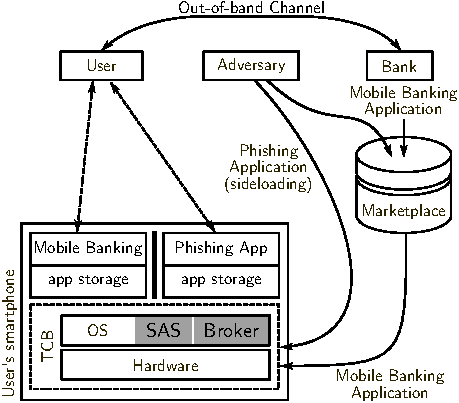
\includegraphics[width=.7\linewidth]{figures/securingphone/phishing_system_model}
    \caption[System model overview]{
    System model overview. Each application running on the smartphone is sandboxed and cannot access the memory or storage of other applications. 
    Applications are installed from the marketplace or via sideloading.
    The bank has an out-of-band channel (e.g., regular mail) to its customers.
    Our protocol adds two components to the platform TCB (shown in gray).
    The \secmodule{} can measure installed applications and has a UI to receive user inputs.
    A Secure Attention Sequence (SAS) is used to start the \secmodule{}.}
    \label{fig:sp_phishing_system-model}
\end{figure}

Since we consider a mobile banking scenario, we assume the existence an out-of-band-channel between the bank (i.e., the application provider) and the user.
An example of this channel is the (regular) mail system routinely used by banks as a secure and authentic channel to transfer PINs and other credentials to their customers.
As currently used to reset forgotten passwords, emails can also be used as an alternative out-of-band channel.

The goal of the adversary is to phish the indicator that the user chooses for the banking application.
We assume that the user has previously installed, either from the marketplace or via sideloading, a malicious application on his smartphone.
Leveraging the malicious application on the user's phone, the adversary can launch any of the attacks presented in Section~\ref{subsec:sp_phishing_attacks}.
However, the adversary cannot compromise the device TCB or the out-of-band channel between the bank and the user.


\subsection{Secure Indicator Setup Protocol}
\label{sec:setup:sp_phishing_protocol}

Setting up an indicator in the presence of malicious software requires the user to identify the banking application for which he is choosing the indicator.
A similarity attack to phish the indicator at setup time may be hard for the user to detect.
Similarly, the marketplace operator may fail to identify phishing applications and block their distribution (see Section~\ref{sec:sp_phishing_comparison}).
We argue that no party but the bank can attest the validity of the banking application for which the user is about to choose the indicator.
For this reason, our protocol relies on a trusted component of the mobile platform that, together with the bank, attests the validity of the banking application installed on the device.

In particular, the trusted component and the bank establish an authentic channel to attest the application.
If attestation is successful, the trusted component provides the application with a PIN known by the user. 
The user can identify the legitimate application, if it shows the correct PIN.

Figure~\ref{fig:sp_phishing_system-model} shows in gray the components that we add to the device TCB.
A system component that we call the \secmodule{} can measure applications (e.g., compute a hash of the application binary and its configuration files) installed on the device and has a UI to receive user inputs.
The mobile OS is also enhanced with a Secure Attention Sequence (SAS), which is a common approach to start a particular software component of a TCB~\cite{gligor87tse, mccune09ndss, libonati11ndss}\footnote{A popular SAS is the ``ctrl-alt-del'' sequence in Windows systems which generates a non-maskable interrupt that starts the user-logon process.}.
We implement the SAS operation as two repeated presses of the home button and we use it to start the \secmodule{}.
When the \secmodule{} is running, the mobile OS ensures that no background application can activate to the foreground.

The bank and the \secmodule{} establish an authentic channel using the out-of-band channel between the bank and the user.
The bank sends a measurement of the legitimate banking application over the authentic channel, so that the \secmodule{} can compare it with the measurement of the banking application installed on
the device. If the two measurements match, the \secmodule{} transfers to the banking application a PIN known by the user.
The banking application shows the PIN to the user who can, therefore, identify the legitimate banking application.

Figure~\ref{fig:sp_phishing_protocol} illustrates the steps to securely setup a personalized indicator. Here we explain them in detail.

\begin{enumerate}
\item The bank uses the out-of-band channel (e.g., regular mail) to send a PIN to the user.

\item The user installs the application, downloading it from the marketplace.
    When the installation completes, the user performs the SAS operation to start the \secmodule{}.
    While the \secmodule{} is running, the mobile OS prevents third-party applications from activating to the foreground.

\item   The user inputs the PIN to the \secmodule{}.

\item   The \secmodule{} and the bank use the PIN to run a Password Authenticated Key Exchange (PAKE)
        protocol~\cite{speke} and establish a shared key.

\item   The bank sends the measurement of the legitimate banking application to the \secmodule{}.
        The measurement can be the hash of the application installation package.
        The message is authenticated using the key established during the previous step.
	
\item   The \secmodule{} verifies the authenticity of the received message, measures the banking application on the device,
        and checks its measurement against the reference value received from the bank.

\item   If the two measurements are identical, the \secmodule{} securely transfers the PIN to the banking application
        (e.g., writes the PIN to the application-specific storage).
        Otherwise the \secmodule{} aborts the protocol and notifies the user.

\item   The \secmodule{} starts the banking application and the mobile OS restores the functionality that allows background applications to
        activate to the foreground. The banking application displays the PIN which serves
        as a confirmation to the user that the application in foreground is the legitimate banking application.

\item   The user identifies the application in foreground as the legitimate banking application if it displays the same PIN that the user has received from the bank.
        At this point, the user can choose a personalized indicator for the banking application.
\end{enumerate}

\begin{figure}[!t]
    \centering
    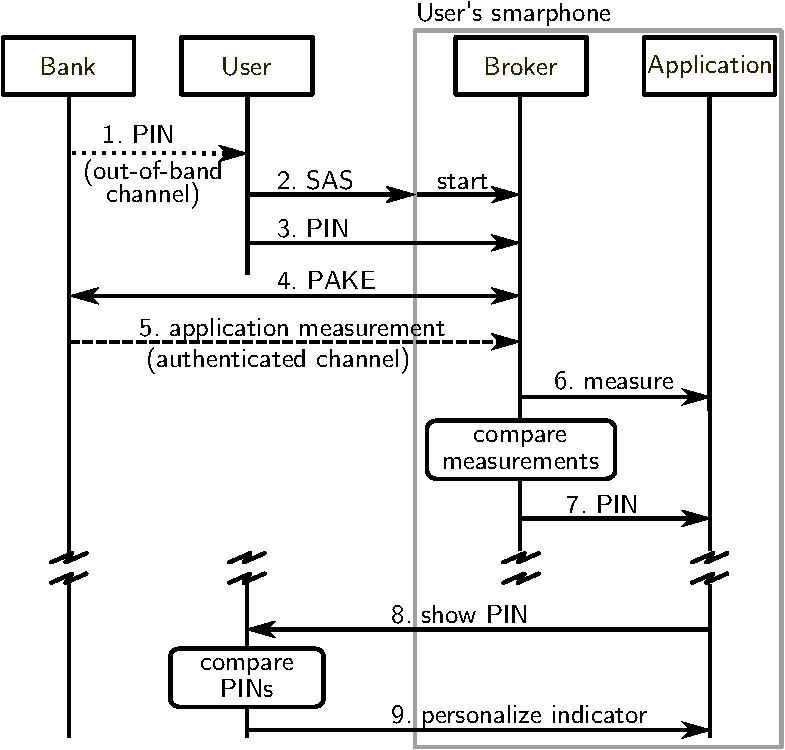
\includegraphics[width=.7\linewidth]{figures/securingphone/phishing_protocol_v3}
    \caption[The personalized indicator setup protocol]{The personalized indicator setup protocol. The user performs an SAS operation to start the \secmodule{} and enters the PIN.
    The \secmodule{} verifies the installed banking application with the help of the bank.
    If the installed application is the legitimate one, the \secmodule{} starts it and the user can choose a custom indicator.}
    \label{fig:sp_phishing_protocol}
\end{figure}

\paragraph{Security Analysis.}

Our protocol relies on the user attention when setting up the indicator.
At the beginning of the setup protocol, the user must input the PIN only after performing the SAS operation.
At the end of the protocol, the user must choose an indicator only if the application in foreground displays the same PIN that the user has received from the bank.

The SAS operation and the device TCB guarantee that no information is leaked when the user inputs the PIN to the \secmodule{}.
In particular, no malicious application can masquerade as the \secmodule{} to phish the PIN.
The PIN is used as a one-time password to derive a key through the PAKE protocol.
The derived key is only used to authenticate one message (from the bank to the \secmodule{}).
The security properties of the PAKE protocol guarantee that, given a transcript of the protocol, the adversary can neither learn the PIN, nor brute-force the set of possible PINs~\cite{spekesec}.

The application-specific storage functionality, provided by the mobile OS, guarantees that the PIN received by the banking application can not be read by
other applications.

A phishing application on the device will not receive the PIN from the \secmodule{} because its measurement differs from the one of the legitimate banking application.
The adversary cannot impersonate the bank to the \secmodule{} without knowledge of either the PIN or the key derived through the PAKE protocol.

\subsection{Implementation}
\label{sec:setup:sp_phishing_implementation}

We build a prototype of our setup protocol for the Android platform.
We use a Samsung Galaxy S3 and develop against the CyanogenMod Android OS (version 4.3 ``JellyBean'').
Cryptographic operations are based on the Bouncy Castle library~\cite{bouncycastle}.
Message authentication uses HMAC-SHA256 with a 128-bit key.
The bank's server is implemented in Python, using the CherryPy Web Framework and SQLite.
Client-server communication works over a standard HTTP channel using messages in the JSON standard format.
Our implementation adds two Java files, to implement the \secmodule{} as a privileged application, and modifies four system Java files.
A total of 652 lines of code were added to the system TCB.

We add an extra tag (\texttt{<secureapk>}) to the Android Manifest file of the banking application.
The tag contains two fields indicating a URL and an application handle.
The \secmodule{} uses the URL to contact the application provider (i.e., the bank) and the handle to identify the application to attest.
When the banking application is installed, the \texttt{PackageParser} of the Android OS reads the extra information in the \texttt{<secureapk>} tag and stores it for later use.

\begin{figure}[!t]
  \centering
  \subfigure[] {%
    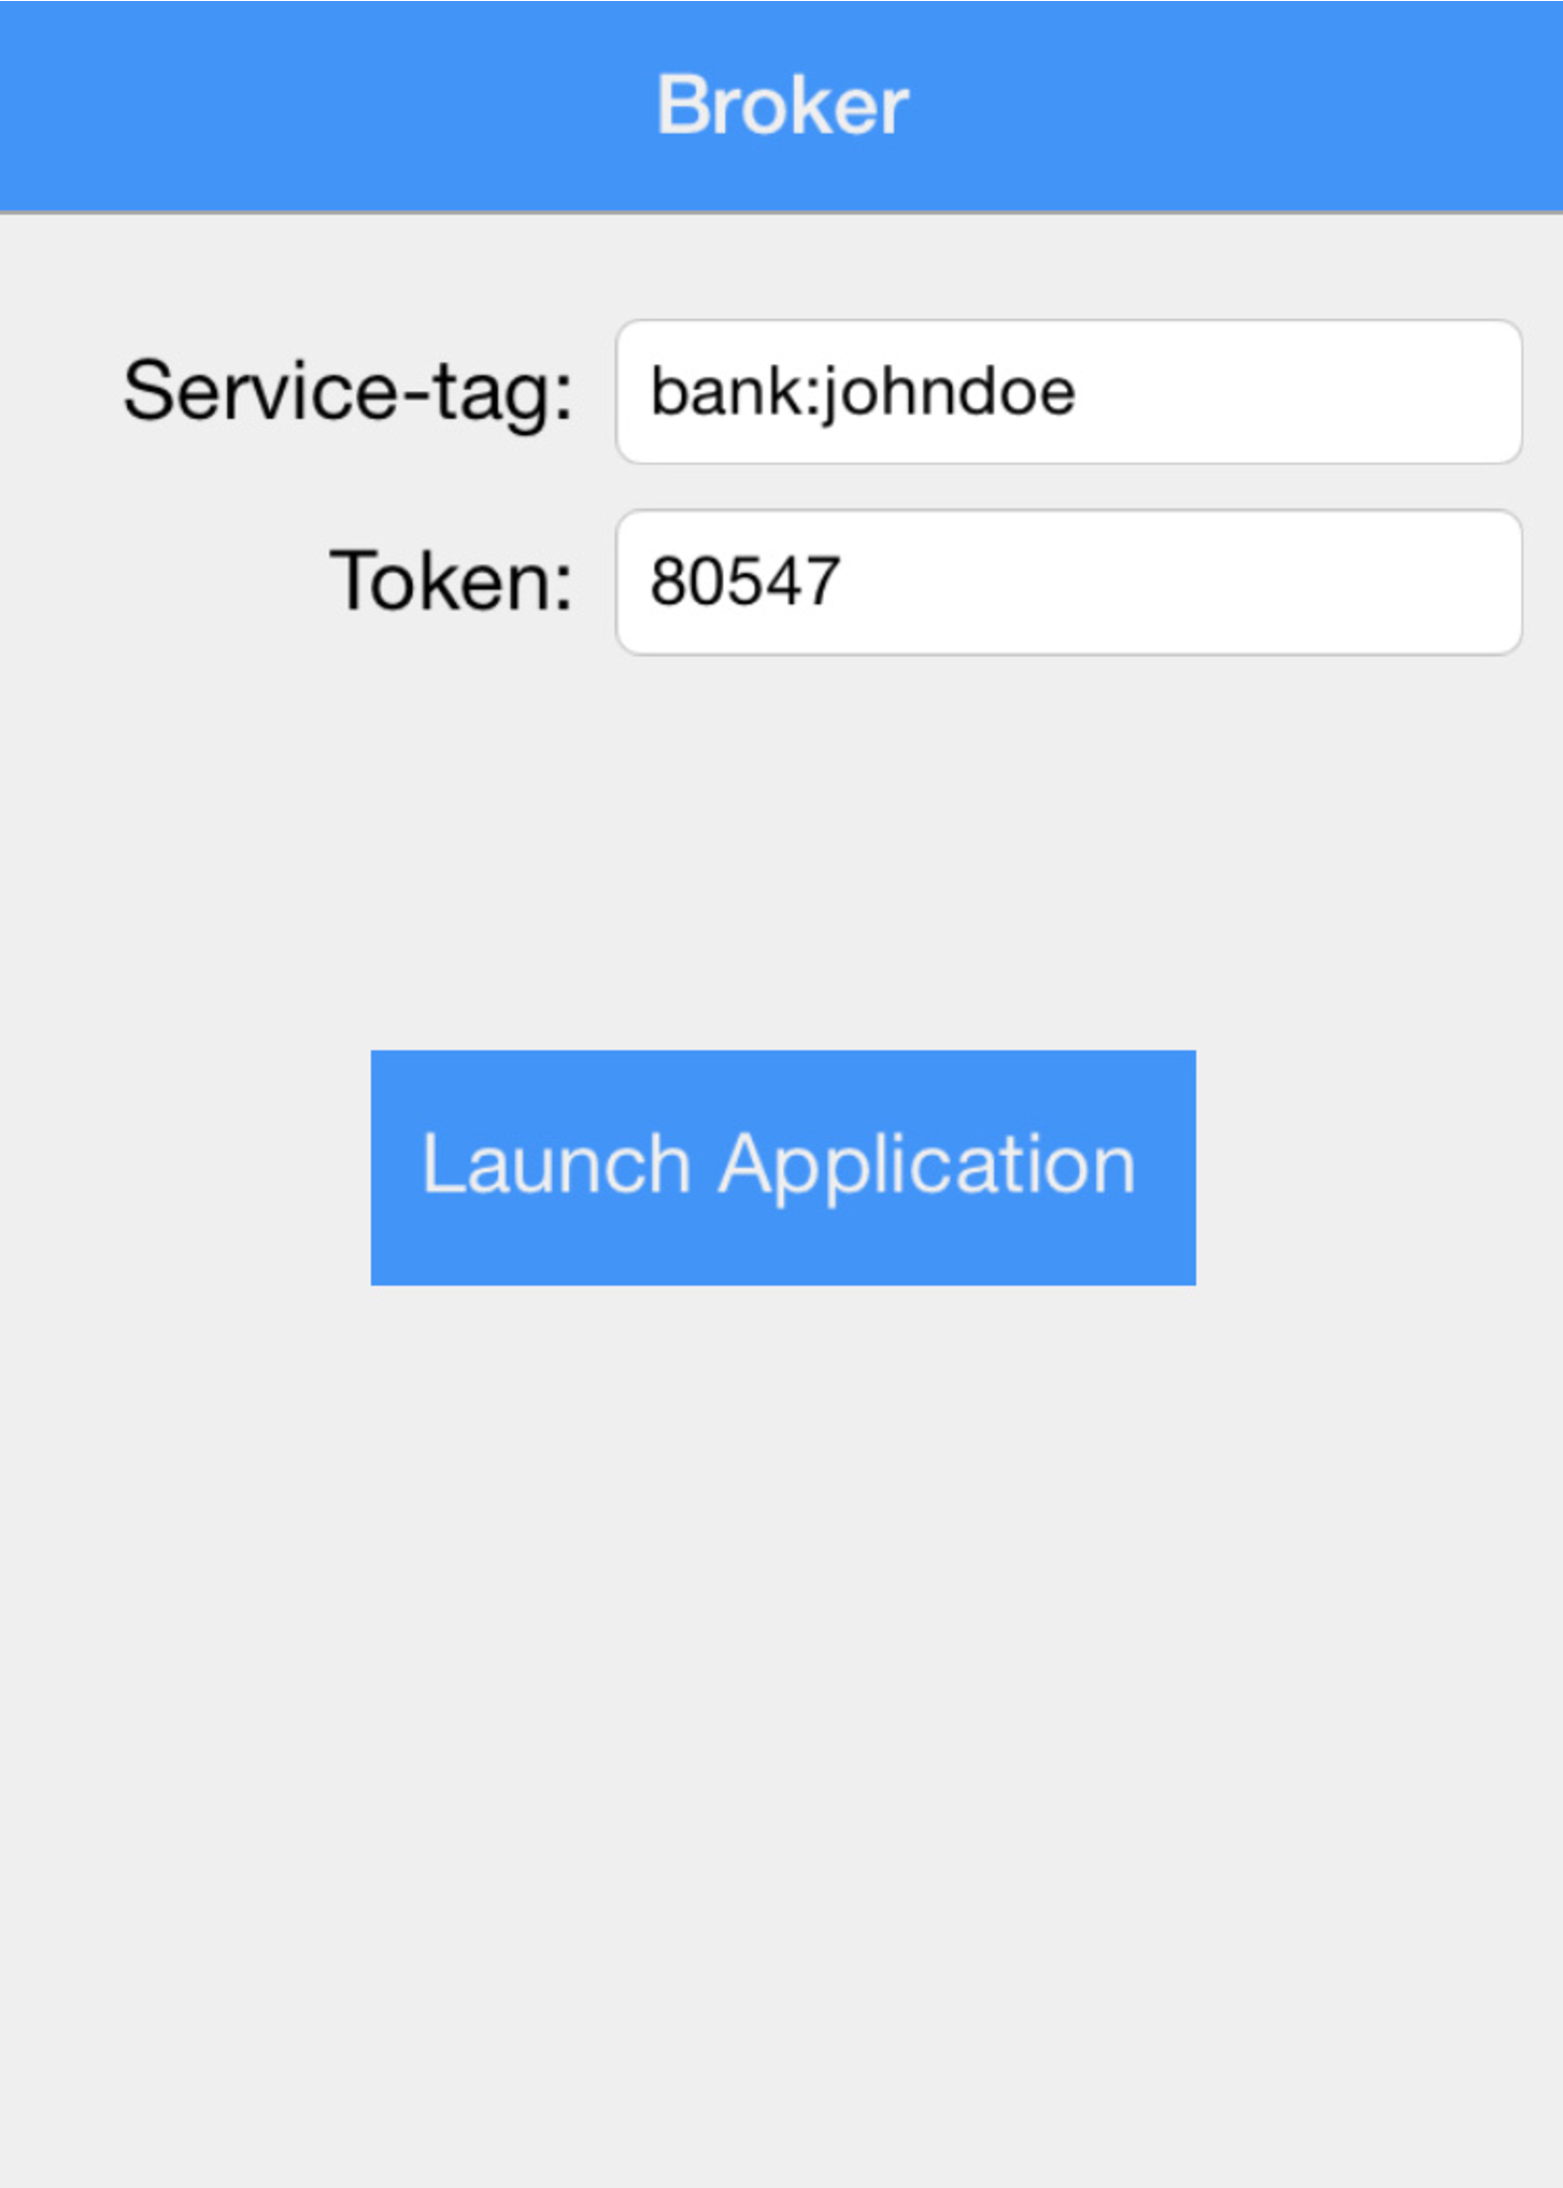
\includegraphics[width=.42\linewidth]{figures/securingphone/phishing_broker_wireframe}
    \label{fig:sp_phishing_broker}
  }
  ~
  \subfigure[]{%
    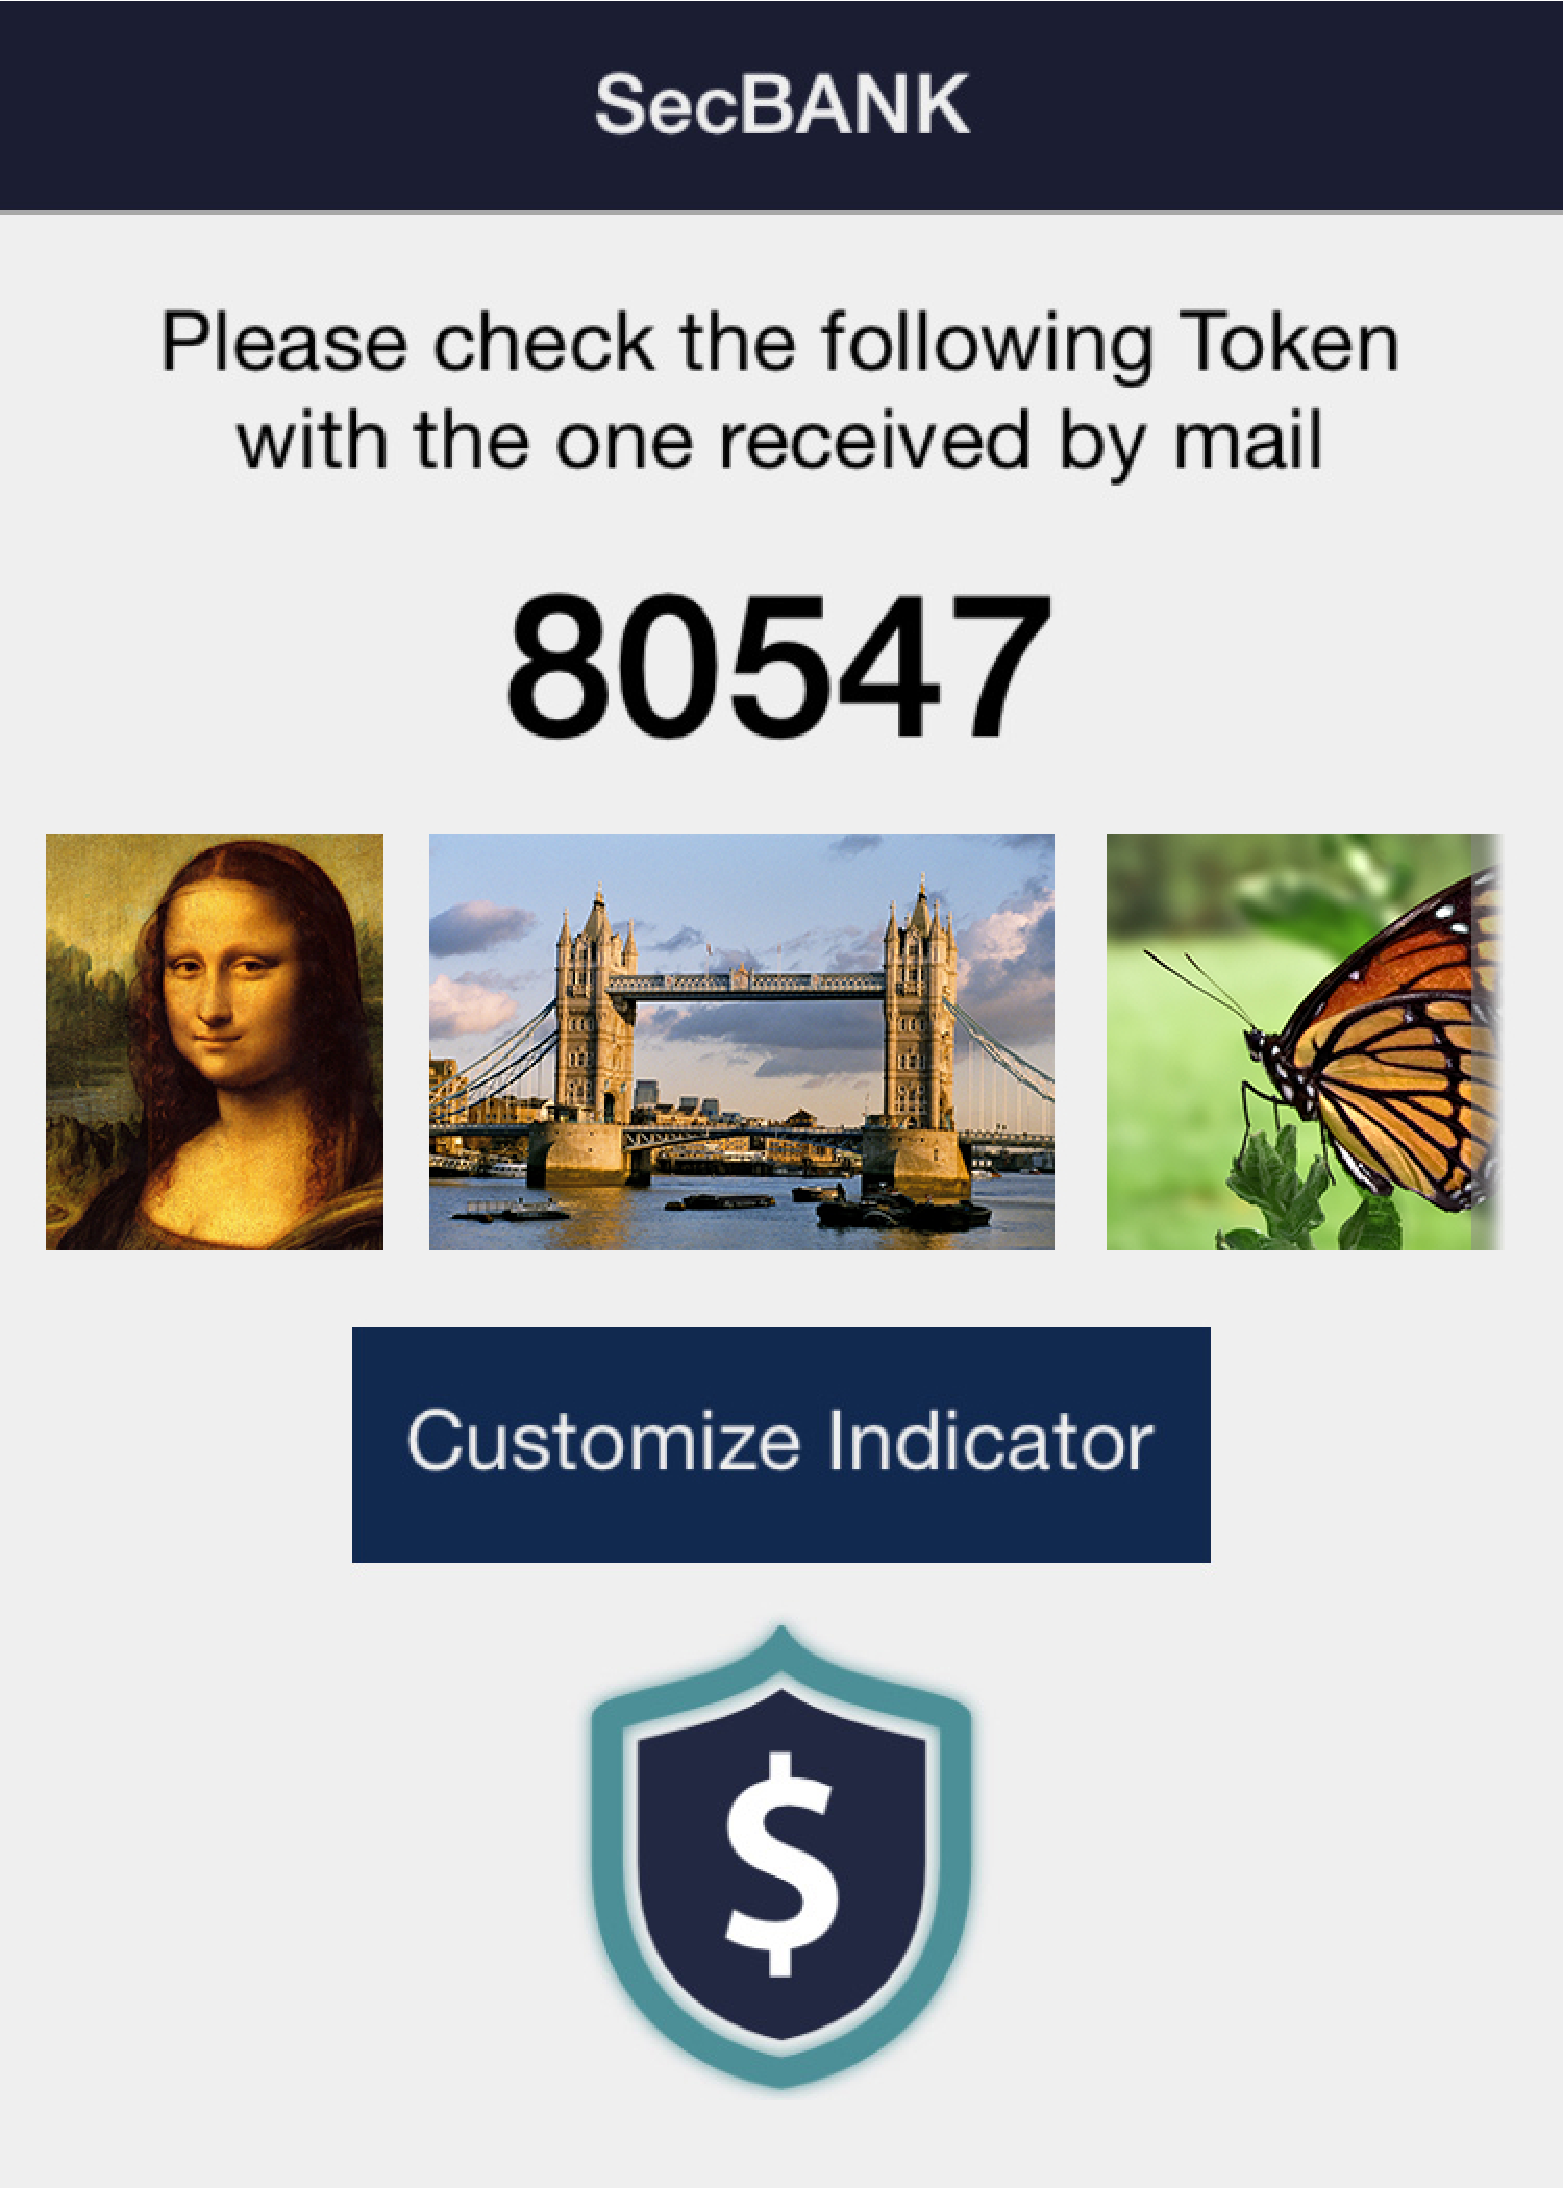
\includegraphics[width=.42\linewidth]{figures/securingphone/phishing_bank_customize.pdf}
    \label{fig:sp_phishing_tokenvoid}
  }
  \caption[\secmodule{} and the Banking application started by it]{
  (a) Screenshot of the \secmodule{} prototype. The user inputs the service tag and the PIN received by the bank.
  (b) Banking application started by the \secmodule{}. The user must verify that the PIN displayed matches the one received by the bank.
  The application shows the images in the local photogallery and the user can select one as the indicator.}
\end{figure}

We assign the SAS operation to a double-tap on the home button.
The SAS operation unconditionally starts the \secmodule{} that asks the user to enter the PIN received from the bank (see Figure~\ref{fig:sp_phishing_broker}).
In our implementation, the bank sends to the user a 5-digits PIN (e.g., ``80547'')
and a \emph{service tag}. The service tag contains an application handle used by the \secmodule{}
to search through the registered handles and to identify the application to attest.
The service tag also contains a user ID, sent to the bank by the \secmodule{}, to retrieve the correct PIN from its database.
An example of a service tag is ``bank:johndoe'', where ``bank'' is the application handle and ``johndoe'' is the user ID.
After the user has input the service tag and the PIN, the \secmodule{} uses the handle to identify the application to attest.
At this time the \secmodule{} also fetches the URL stored by the \texttt{PackageParser}, to contact the bank's server.

We use SPEKE~\cite{speke} as an instantiation of the key establishment protocol.
SPEKE uses 4 messages, including a key confirmation step.
The first SPEKE message sent by the \secmodule{} also contains the user ID that allows the bank's server to select the correct PIN from its database.
The server uses the key established via the PAKE protocol to compute a MAC over the hash of the legitimate application.
Both the hash and the authentication tag are sent to the \secmodule{}.
The \secmodule{} verifies the authentication tag, hashes the installed application, and compares the hash computed locally with the
received one. If the two hashes match, the \secmodule{} writes the PIN to the application's folder so that it can only be read by
that application. Otherwise, the \secmodule{} aborts and notifies the user.

Figure~\ref{fig:sp_phishing_tokenvoid} shows the banking application started by the \secmodule{}.
The user is asked to compare the displayed PIN with the one received via mail and choose a personalized indicator.

\paragraph{Evaluation.}

\begin{table}[!t]
  {\small
  \begin{center}
    {\tabulinesep=.6mm
      \setlength{\tabcolsep}{1.5mm}
      \begin{tabu}{|l|l|} \hline
        TCB increment           & 652 LoC \\ \hline
        Communication overhead  & 705 bytes \\ \hline
        Execution time (WiFi)   & 421ms ($\pm$21ms)\\
        Execution time (3G)     & 2042ms ($\pm$234ms)\\
        Execution time (Edge)   & 2957ms ($\pm$303ms)\\ \hline
      \end{tabu}}
  \end{center}}
  \caption[Evaluation summary for the personalized indicator setup prototype]{Evaluation summary for the personalized indicator setup prototype.}
  \label{tab:sp_phishing_implementation}
\end{table}

We evaluate the setup protocol using a a sample banking application of 264KB.
Client-server communication overhead totals to 705 bytes, of which 641 bytes account for the SPEKE protocol. (Communication overhead is independent of the size of the application.)
We test the protocol over a WiFi connection (hosting the server in a remote location, i.e., not on a local network), as well as over 3G and EDGE cellular data connections.
Table~\ref{tab:sp_phishing_implementation} summarizes the evaluation in terms of added lines of code, communication overhead, and execution time.
We note that hashing the banking application takes  25ms on average, with a standard deviation of 2ms.
The time to hash an application increases linearly with the size of the application and remains lower than the network delay for applications up to 100MB.

\subsection{Usability}
\label{sec:setup:sp_phishing_usability}
We run a small-scale user study to evaluate the usability of our setup protocol.
In particular, our goal was to understand how easy it is for users to setup indicators by following written instructions, like the ones a bank customer would receive from his bank.
We also wanted to verify how attentive users are when comparing the PIN shown by the application with the one received from the bank.

We invited participants to our lab and asked them to carry out the setup protocol as if they were customers of a bank that uses indicators in its application.
We provided participants with a phone and a letter from the bank with instructions on how to setup the indicator. A sample letter can be found in Appendix~\ref{app:sp_phishing_bankletter}
We assigned participants to three different groups.
One group carried out the set up protocol in benign settings.
For the remaining two groups, we simulated variants of a background attack at the time when the banking application displays the PIN (step 8 of the setup protocol).
We recorded whether participants pressed the ``Customize Indicator'' button and chose a personalized indicator while under attack.


\paragraph{Procedure.}

We advertised the study as a user study ``to evaluate the usability of a setup protocol for an e-banking application''.
Participants were asked to come to our lab and setup the application on a smartphone that we provided.
We informed participants that we would not collect any personal information and offered a compensation of CHF 20.-.

We selected 30 participants and assigned them to one of three groups in a round-robin fashion. (None of these participants were involved in the user study of Section~\ref{sec:sp_phishing_userstudy}.)
The difference among the groups was the PIN shown by the banking application right before participants were asked to choose a personalized indicator.
Group A participants were shown the same PIN that appeared  on the letter from the bank.
Group B participants were shown a random PIN.
Group C participants where shown no PIN.

Participants of group A reflected the user experience of the setup protocol under no attack.
Participants of groups B and C reflected the user experience of the setup protocol under a background attack.


\emph{Experiment.}
The experiment started with a pre-test questionnaire to collect demographic information.
After the questionnaire, participants were given a smartphone and  a letter from a fictitious bank with instructions to setup the indicator.
The letter included a 5-digit PIN and a service tag to be used during the setup protocol.
The procedure was the one described in Section~\ref{sec:setup:sp_phishing_protocol} and was carried out on a Galaxy S3.
We stress that we did not interact with the participants for the duration of the setup protocol.
Participants were also asked to fill in a post-test questionnaire to evaluate the procedure they had just completed.

\paragraph{Results.}

\begin{figure}[!ht]
	\centering
	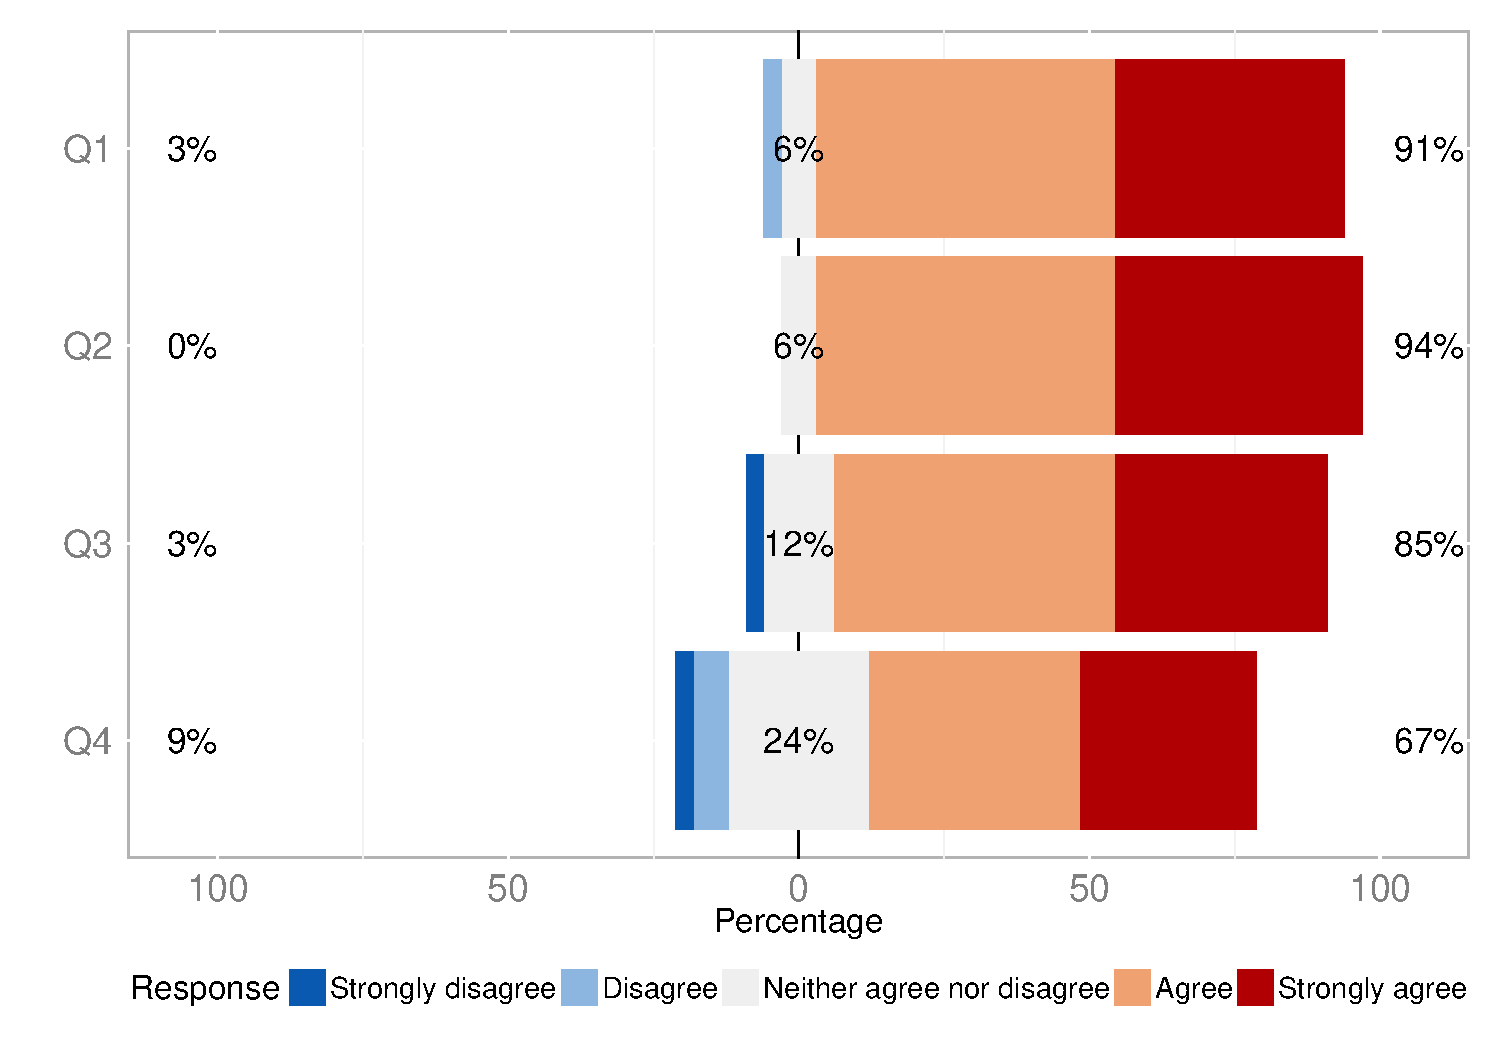
\includegraphics[width=.8\columnwidth]{figures/securingphone/phishing_second_likert}
	\caption[Answers to the post-test questionnaire for the user study on the indicator setup protocol]{
    Answers to the post-test questionnaire for the user study on the indicator setup protocol.
	Percentages on the left side include participants that answered ``Strongly disagree'' or ``Disagree''.
	Percentages in the middle account for participants that answered ``Nor agree, nor disagree''.
	Percentages on the right side include participants that answered ``Agree'' or ``Strongly agree''.}
	\label{plot:sp_phishing_second_likert}
\end{figure}

37\% participants were males and 63\% were females. Most of them had completed a university degree (73\%), and were aged between 24 and 35 (80\%).

All participants in group A managed to complete the task successfully.
All participants of group B aborted the setup procedure because they detected a mismatch between the PIN displayed by the banking application and the one in the letter from the bank.
40\% percent of the participants in group C failed to detect the missing PIN and completed the setup process, thereby leaking the indicator to the phishing application.

The post-test questionnaire revealed that 91\% of the participants rated the instruction sheet easy to understand (Q1) and 94\% of them rated the task easy to complete (Q2).
85\% of the participants believed that they had completed the task successfully (Q3) and 67\%  of them would use the mechanism in a mobile banking application (Q4).
Figure~\ref{plot:sp_phishing_second_likert} shows the distribution of the answers.
Appendix~\ref{app:sp_phishing_posttestII} provides the full text of items Q1--Q4.

Our study suggests that the setup procedure was simple enough to be completed by average users.
Regarding attack detection, the ``missing PIN'' attack was the only one that went undetected.
Participants may have judged the absence of the PIN as a temporary bug and decided to continue with the setup protocol.
Similarly to what we have reported in Section~\ref{sec:sp_phishing_discussion}, this result shows that users are acquainted with software bugs and
are likely to tolerate a temporary bug even during a security-sensitive operation.
Nevertheless, the user study reveals that our solution is usable and effective.

\section{Related Work}

In chapter~\ref{chap:sp_relatedwork} we discussed smartphone malware attacks and countermeasures in general. In the following we review related work that looks at phishing attacks, in particular.

A systematic evaluation of application phishing attacks was recently provided in~\cite{bianchi15sp}. The authors use static analysis to detect applications
that use APIs that enable certain classes of application phishing attacks.
They also introduce an on-device solution that allows users to identify applications with which they are interacting.
In the proposed solution, the OS displays a status bar that shows the application and developer names together with an image chosen by the user.
The image, therefore, is used by the user to tell the authentic status bar managed by the OS from a fake status bar that a phishing application can show if it gains control of the entire screen.
Compared to personalized indicators, the proposed solution incurs more deployment costs, since it requires changes to the OS and the marketplace.
The authors of~\cite{bianchi15sp} also use Amazon Mechanical Turk to run a user study with 304 participants, and assess the effectiveness of phishing attacks in mobile platforms. 
The user study corroborates our findings on personalized indicators, although the authors placed the image in the navigation bar rather than in the application itself. 
Furthermore, the user study in~\cite{bianchi15sp} was a one-off test that did not last for a week and, compared to ours, let participants interact with an emulated android device through a web-browser rather then letting participants use their phones in their own typical setting.

Anti-phishing techniques for the web have been deployed in practice~\cite{dhamija06chi,hong12cacm}.
Proposals include automated comparison of website URLs~\cite{maurer-css12},
visual comparison of website contents~\cite{chen10tit, yue-www07},
use of a separate and trusted authentication device~\cite{parno06fc},
personalized indicators~\cite{dhamija05soups,schechter07sp,lee-w2sp14},
multi-stage authentication~\cite{herzberg12},
and attention key sequences to trigger security checks on websites~\cite{wu-soups06}.
While some of these mechanisms are specific to the web environment, others could be adapted also for mobile application phishing detection. Website phishing in the context of mobile web
browsers has been studied in~\cite{niu-upsec08,rydstedt-woot10}.

Finally, we focus on previous research that studied the effectiveness of security indicators. These work have mostly focused on phishing on the web.
Studies in this context have shown that users tend to ignore security indicators such as personalized images~\cite{schechter07sp,lee-w2sp14} or toolbars~\cite{wu-chi06, jackson-fincrypto07}.
Browser warnings have been evaluated positively in a recent work~\cite{akhawe13usenix}, even if previous studies suggest otherwise~\cite{sunshine-usenix09,egelman2008chi,dhamija06chi}. In the context of mobile browsers, a recent work~\cite{traynorimc} further showed how the situation is worse than for desktop browsers.

\section{Summary and Future Work}

Despite the security mechanisms used in modern smartphones, it is still possible for an attacker to install a malicious application on his victims' phones. In this chapter we looked at application phishing attacks in detail. Such attacks are an emerging threat for mobile application platforms and the first successful attacks have already caused significant financial losses.

We first analyzed possible ways in which a phishing application can fool the victim and steal his credentials. When listing possible countermeasures against phishing attacks we noticed that no single one could protect against all types of attacks. We focused our attention on personalized indicators, which are easy to deploy and are a well-known countermeasure to address the problem of phishing. Previous studies in the context of websites have shown that indicators fail to prevent the majority of attacks. Consequently, the research community has deemed personalized indicators an ineffective anti-phishing mechanism. In this chapter we reported our findings from the first user study on smartphones that evaluates the effectiveness of personalized security indicators for mobile applications. Our results show a clear improvement over the previous studies, which gives us reason to believe that indicators, when applied to an appropriate context, may be more effective than their current reputation suggests. We conclude that the research community should revisit the question of personalized indicator effectiveness and further studies are needed to fully understand their benefits in new deployment contexts such as in mobile applications. Finally, we proposed a secure setup protocol for personalized security indicators.

\subsection{Future Work}

We presented a first user study on how security indicators in the new context of mobile applications can help detect application phishing attacks. We now discuss interesting directions for future research.

\paragraph{Bank Deployment.} 
Our user study is based on a mobile banking application we developed. We could not replicate previous studies that used clients of a real bank that uses security indicators. One direction for future work is to collaborate with a banking institution to study the effectiveness of personalized security indicators in a real deployment. This would allow the study to last longer and target a varied population of users.

\paragraph{Personalized Security Indicators.}
In our user study we allowed participants to choose an indicator from their photo gallery. The indicator was then placed prominently on the login screen. Future user studies could look at different indicator size and position. Furthermore one could further evaluate the effectiveness of different indicator types such as interactive indicators. Interactive indicators require the user to not only assess their presence but also interact with them in some manner, such as for example tapping on them or swiping across them. 

\paragraph{User Perception.}
An interesting research direction is to study how much users understand changes in user interfaces. This is of particular interest in case that a solution that compares applications UIs is used to detect phishing attacks. Such a solution is fooled by an attacker that changes slightly the appearance of the malicious application. The question that needs to be answered is how much can one change the UI of an application before users would not enter their credentials anymore.